%% USPSC-TCC-modelo-ICMC.tex
% ---------------------------------------------------------------
% USPSC: Modelo de Trabalho Academico (tese de doutorado, dissertacao de
% mestrado e trabalhos monograficos em geral) em conformidade com 
% ABNT NBR 14724:2011: Informacao e documentacao - Trabalhos academicos -
% Apresentacao
%----------------------------------------------------------------
%% Esta é uma customização do abntex2-modelo-trabalho-academico.tex de v-1.9.5 laurocesar 
%% para as Unidades do Campus USP de São Carlos:
%% EESC - Escola de Engenharia de São Carlos
%% IAU - Instituto de Arquitetura e Urbanismo
%% ICMC - Instituto de Ciências Matemáticas e de Computação
%% IFSC - Instituto de Física de São Carlos
%% IQSC - Instituto de Química de São Carlos
%%
%% Este trabalho utiliza a classe USPSC.cls que é mantida pela seguinte equipe:
%% 
%% Programação:
%%   - Marilza Aparecida Rodrigues Tognetti - marilza@sc.usp.br (PUSP-SC)
%%   - Ana Paula Aparecida Calabrez - aninha@sc.usp.br (PUSP-SC)
%% Normalização e Padronização:
%%   - Brianda de Oliveira Ordonho Sigolo - brianda@usp.br (IAU)
%%   - Elena Luzia Palloni Gonçalves - elena@sc.usp.br (EESC)
%%   - Eliana de Cássia Aquareli Cordeiro - eliana@iqsc.usp.br (IQSC)
%%   - Flávia Helena Cassin - cassinp@sc.usp.br (EESC)
%%   - Maria Cristina Cavarette Dziabas - mcdziaba@ifsc.usp.br (IFSC)
%%   - Regina Célia Vidal Medeiros - rcvmat@icmc.usp.br (ICMC)
%%
%% O USPSC-modelo.tex utiliza:	
%%  USPSC.cls e USPSC1.cls
%% 	USPSC-modelo-references.bib
%%	USPSC-modelo.tex
%%	USPSC-unidades.tex
%%	Um dos arquivos com dados pre-textuais abaixo, em conformidade com a Unidade de vínculo do autor:
%%				USPSC-pre-textual-EESC.tex
%%				USPSC-pre-textual-IAU.tex
%%				USPSC-pre-textual-ICMC.tex
%%				USPSC-pre-textual-IFSC.tex
%%				USPSC-pre-textual-IQSC.tex
%%				USPSC-pre-textual-OUTRO.tex
%%	USPSC-fichacatalografica.tex ou fichacatalografica.pdf
%%	folhadeaprovacao.pdf
%%	USPSC-Cap1-Introducao.tex
%%	USPSC-Cap2-Desenvolvimento.tex
%%	USPSC-Cap3-Citacoes.tex
%%	USPSC-Cap4-referencias.tex
%%	USPSC-Cap5-Conclusao.tex
%%	USPSC-Apendices.tex
%%	USPSC-Anexos.tex
%%	USPSC-AcentuacaoLaTeX.tex
%%	USPSC-LetrasGregas.tex
%%	USPSC-SimbolosUteis.tex

%----------------------------------------------------------------
%% Sobre a classe abntex2.cls:
%% abntex2.cls, v-1.9.5 laurocesar
%% Copyright 2012-2015 by abnTeX2 group at https://www.abntex.net.br/ 
%%
%----------------------------------------------------------------

\documentclass[
% -- opções da classe memoir --
12pt,		% tamanho da fonte
openright,	% capítulos começam em pág ímpar (insere página vazia caso preciso)
twoside,  % para impressão em anverso (frente) e verso. Oposto a oneside - Nota: utilizar \imprimirfolhaderosto*
%oneside, % para impressão em páginas separadas (somente anverso) -  Nota: utilizar \imprimirfolhaderosto
% inclua uma % antes do comando twoside e exclua a % antes do oneside 
a4paper,			% tamanho do papel. 
% -- opções da classe abntex2 --
chapter=TITLE,		% títulos de capítulos convertidos em letras maiúsculas
% -- opções do pacote babel --
english,			% idioma adicional para hifenização
french,				% idioma adicional para hifenização
spanish,			% idioma adicional para hifenização
brazil				% o último idioma é o principal do documento
% {USPSC} configura o cabeçalho contendo apenas o número da página
]{USPSC}
%]{USPSC1}
% Inclua % antes de ]{USPSC} e retire a % antes de %]{USPSC1}
% para utilizar o cabeçalho diferenciado para as páginas pares e ímpares como indicado abaixo:
%- páginas ímpares: cabeçalho com seções ou subseções e o número da página
%- páginas pares: cabeçalho com o número da página e o título do capítulo 
% ---

% ---
% Pacotes básicos - Fundamentais 
% ---
\usepackage[T1]{fontenc}		% Seleção de códigos de fonte.
\usepackage[utf8]{inputenc}		% Codificação do documento (conversão automática dos acentos)
\usepackage{lmodern}			% Usa a fonte Latin Modern
% Para utilizar a fonte Times New Roman, inclua uma % no início do comando acima  "\usepackage{lmodern}"
% Abaixo, tire a % antes do comando  \usepackage{times}
%\usepackage{times}		    	% Usa a fonte Times New Roman	
% Lembre-se de alterar a fonte no comando que imprime o preâmbulo no arquivo da Classe USPSC.cls				
\usepackage{lastpage}			% Usado pela Ficha catalográfica
\usepackage{indentfirst}		% Indenta o primeiro parágrafo de cada seção.
\usepackage{color}				% Controle das cores
\usepackage{graphicx}			% Inclusão de gráficos
\usepackage{float} 				% Fixa tabelas e figuras no local exato
%\usepackage{chemfig,chemmacros} % Para escrever reações químicas
\usepackage{microtype} 			% para melhorias de justificação
\usepackage{pdfpages}
\usepackage{makeidx}            % para gerar índice remissimo
% ---

% ---
% Pacotes de citações
% Citações padrão ABNT
% ---
% Sistemas de chamada: autor-data ou numérico.
% Sistema autor-data
\usepackage[alf,abnt-emphasize=bf, abnt-thesis-year=both, abnt-repeated-author-omit=yes, abnt-last-names=abnt, abnt-etal-cite,abnt-etal-list=3, abnt-etal-text=default, abnt-and-type=e, abnt-doi=doi, abnt-url-package=none, abnt-verbatim-entry=no]{abntex2cite}

% Para o IQSC, que indica todos os autores nas referências, incluir % no início do comando acima e retirar a % do comando abaixo 

%\usepackage[alf,abnt-emphasize=bf, abnt-thesis-year=both, abnt-repeated-author-omit=yes, abnt-last-names=abnt, abnt-etal-cite,abnt-etal-list=0, abnt-etal-text=default, abnt-and-type=e]{abntex2cite}

% Sistema Numérico
% Para citações numéricas, sistema adotado pelo IFSC, incluir % no início do comando acima e retirar a % do comando abaixo 
%\usepackage[num,overcite,abnt-emphasize=bf, abnt-thesis-year=both, abnt-repeated-author-omit=yes, abnt-last-names=abnt, abnt-etal-cite,abnt-etal-list=0, abnt-etal-text=default, abnt-and-type=e]{abntex2cite}

% Complementarmente, verifique as instruções abaixo sobre os Pacotes de Nota de rodapé
% ---
% Pacotes de Nota de rodapé
% Configurações de nota de rodapé

% O presente modelo adota o formato numérico para as notas de rodapés quando utiliza o sistema de chamada autor-data para citações e referências. Para utilizar o sistema de chamada numérico para citações e referências, habilitar um dos comandos abaixo.
% Há diversa opções para nota de rodapé no Sistema Numérico.  Para o IFSC, habilitade o comando abaixo.

%\renewcommand{\thefootnote}{\fnsymbol{footnote}}  %Comando para inserção de símbolos em nota de rodapé

% Outras opções para nota de rodapé no Sistema Numérico:
%\renewcommand{\thefootnote}{\alph{footnote}}      %Comando para inserção de letras minúscula em nota de rodapé
%\renewcommand{\thefootnote}{\Alph{footnote}}      %Comando para inserção de letras maiúscula em nota de rodapé
%\renewcommand{\thefootnote}{\roman{footnote}}     %Comando para inserção de números romanos minúsculos  em nota de rodapé
%\renewcommand{\thefootnote}{\Roman{footnote}}     %Comando para inserção de números romanos minúsculos  em nota de rodapé

\renewcommand{\footnotesize}{\small} %Comando para diminuir a fonte das notas de rodapé

 % ---
 % Pacote para agrupar a citação numérica consecutiva
 % Quando for adotado o Sistema Numérico, a exemplo do IFSC, habilite 
 % o pacote cite abaixo retirando a porcentagem antes do comando abaixo
 %\usepackage[superscript]{cite}	

% ---
% Pacotes adicionais, usados apenas no âmbito do Modelo Canônico do abnteX2
% ---
\usepackage{lipsum}				% para geração de dummy text
% ---




% pacotes de tabelas
\usepackage{multicol}	% Suporte a mesclagens em colunas
\usepackage{multirow}	% Suporte a mesclagens em linhas
\usepackage{longtable}	% Tabelas com várias páginas
\usepackage{threeparttablex}    % notas no longtable
\usepackage{array}

% ---
% DADOS INICIAIS - Define sigla com título, área de concentração e opção do Programa 
% Consulte a tabela referente aos Cursos de Graduação de sua unidade contante do
% arquivo USPSC-TCC-Siglas estabelecidas para as Graduações por Unidade.xlsx 
% ou no APÊNDICES G
\siglaunidade{ICMC-TCC}
\programa{MBACD}
% Os demais dados deverão ser fornecidos no arquivo USPSC-pre-textual-UUUU ou USPSC-TCC-pre-textual-UUUU, onde UUUU é a sigla da Unidade. 
% Exemplo:USPSC-pre-textual-IFSC.tex
% ---
% Configurações de aparência do PDF final
% alterando o aspecto da cor azul
\definecolor{blue}{RGB}{41,5,195}

% informações do PDF
\makeatletter
\hypersetup{
	%pagebackref=true,
	pdftitle={\@title}, 
	pdfauthor={\@author},
	pdfsubject={\imprimirpreambulo},
	pdfcreator={LaTeX with abnTeX2},
	pdfkeywords={abnt}{latex}{abntex}{USPSC}{trabalho acadêmico}, 
	colorlinks=true,       		% false: boxed links; true: colored links
	linkcolor=blue,          	% color of internal links
	citecolor=blue,        		% color of links to bibliography
	filecolor=magenta,      		% color of file links
	urlcolor=blue,
	bookmarksdepth=4
}
\makeatother
% --- 
% --- 
% Espaçamentos entre linhas e parágrafos 
% --- 

% O tamanho do parágrafo é dado por:
\setlength{\parindent}{1.3cm}

% Controle do espaçamento entre um parágrafo e outro:
\setlength{\parskip}{0.2cm}  % tente também \onelineskip

% ---
% compila o sumário e índice
\makeindex
% ---

% ----
% Início do documento
% ----
\begin{document}

% Seleciona o idioma do documento (conforme pacotes do babel)
\selectlanguage{brazil}
% Se o idioma do texto for inglês, inclua uma % antes do 
%      comando \selectlanguage{brazil} e 
%      retire a % antes do comando abaixo
%\selectlanguage{english}

% Retira espaço extra obsoleto entre as frases.
\frenchspacing 

% --- Formatação dos Títulos
\renewcommand{\ABNTEXchapterfontsize}{\fontsize{12}{12}\bfseries}
\renewcommand{\ABNTEXsectionfontsize}{\fontsize{12}{12}\bfseries}
\renewcommand{\ABNTEXsubsectionfontsize}{\fontsize{12}{12}\normalfont}
\renewcommand{\ABNTEXsubsubsectionfontsize}{\fontsize{12}{12}\normalfont}
\renewcommand{\ABNTEXsubsubsubsectionfontsize}{\fontsize{12}{12}\normalfont}


% ----------------------------------------------------------
% ELEMENTOS PRÉ-TEXTUAIS
% ----------------------------------------------------------
% ---
% Capa
% ---
\imprimircapa
% ---
% Folha de rosto
% (o * indica impressão em anverso (frente) e verso )
% ---
\imprimirfolhaderosto*
%\imprimirfolhaderosto
% ---
% ---
% Inserir a ficha catalográfica em pdf
% ---
% A biblioteca da sua Unidade lhe fornecerá um PDF com a ficha
% catalográfica definitiva. 
% Quando estiver com o documento, salve-o como PDF no diretório
% do seu projeto como fichacatalografica.pdf e iclua o arquivo
% utilizando o comando abaixo:
%\includepdf{USPSC-Tese-pre-textual/fichacatalografica.pdf} 
% Se você optar por elaborar a ficha catalográfica, deverá 
% incluir uma % antes da linha % antes
% do comando \include{USPSC-Tese-pre-textual/USPSC-fichacatalografica} 
% e retirar o % do comando abaixo


\includepdf{PaginaEmBranco.pdf}

% ---
% Inserir a ficha bibliografica
% ---
% Isto é um exemplo de Ficha Catalográfica, ou ``Dados internacionais de
% catalogação-na-publicação''. Você pode utilizar este modelo como referência. 
% Porém, provavelmente a biblioteca da sua universidade lhe fornecerá um PDF
% com a ficha catalográfica definitiva após a defesa do trabalho. Quando estiver
% com o documento, salve-o como PDF no diretório do seu projeto e substitua todo
% o conteúdo de implementação deste arquivo pelo comando abaixo:
%
\begin{fichacatalografica}
	\hspace{-1.4cm}
	\imprimirnotaautorizacao \\ \\
	%\sffamily
	\vspace*{\fill}					% Posição vertical
	\begin{center}					% Minipage Centralizado
		\imprimirnotabib \\
\begin{table}[htb]
	\scriptsize
	\centering	
	\begin{tabular}{|p{0.9cm} p{8.7cm}|}
		\hline
	      & \\
		  &	  \imprimirautorficha     \\
		
		 \imprimircutter & 
							\hspace{0.4cm}\imprimirtitulo~  / ~\imprimirautor~ ;  ~\imprimirorientadorcorpoficha. -- 	\imprimirlocal, \imprimirdata.   \\
		
		  &  % Para incluir nota referente à versão corrigida no corpo da ficha,
			  % incluir % no início da linha acima e tirar a % do início da linha abaixo
			  %	\hspace{0.4cm} \imprimirtitulo~  / ~\imprimirautor~ ; ~\imprimirorientadorcorpoficha~- ~\imprimirnotafolharosto. -- \imprimirlocal, \imprimirdata.  \\
		
			\hspace{0.4cm}\pageref{LastPage} p. : il. (algumas color.) ; 30 cm.\\ 
		  & \\
		  & 
		    \hspace{0.4cm}\imprimirnotaficha ~--~ 
						  \imprimirunidademin, 
						  \imprimiruniversidademin, 
		                  \imprimirdata. \\ 
		  & \\                 
		   % Para incluir nota referente à versão corrigida em notas,
		    % incluir uma % no início da linha acima e	
		    % tirar a % do início da linha abaixo
		    % & \hspace{0.4cm}\imprimirnotafolharosto \\ 
		  & \\ 
		  & \hspace{0.4cm}1. Ciência de Dados. 2. Aprendizagem de máquina. 3.Cinema 4.Modelos de classificação.  I. \imprimirorientadorficha. 
		   II. Título. \\
	
		     %Se houver co-orientador, inclua % antes da linha (antes de II. Título.) 
		     %          e tire a % antes do comando abaixo 
		     %III. Título. \\   
		  \hline
	\end{tabular}
\end{table}
	\end{center}
\end{fichacatalografica}
% ---




\includepdf{PaginaEmBranco.pdf}
% As informações que compõem a ficha catalográfica estão 
% definidos no arquivo USPSC-pre-textual-UUUU.tex
% ---
% ---
% Inserir errata
% ---

% \begin{errata}
% 	\OnehalfSpacing 			
% 	A errata é um elemento opcional, que consiste de uma lista de erros da obra, precedidos pelas folhas e linhas onde eles ocorrem e seguidos pelas correções correspondentes. Deve ser inserida logo após a folha de rosto e conter a referência do trabalho para facilitar sua identificação, conforme a ABNT NBR 14724 \cite{nbr14724}.
	
% 	Modelo de Errata:
		
% 	\begin{flushleft} 
% 			\setlength{\absparsep}{0pt} % ajusta o espaçamento da referência	
% 			\SingleSpacing 
% 			\imprimirautorabr~ ~\textbf{\imprimirtitulo}.	\imprimirdata. \pageref{LastPage}p. 
% 			%Substitua p. por f. quando utilizar oneside em \documentclass
% 			%\pageref{LastPage}f.
% 			\imprimirtipotrabalho~-~\imprimirinstituicao, \imprimirlocal, \imprimirdata. 
%  	\end{flushleft}
% \vspace{\onelineskip}
% \OnehalfSpacing 
% \center
% \textbf{ERRATA}
% \vspace{\onelineskip}
% \OnehalfSpacing 
% \begin{table}[htb]
% 	\center
% 	\footnotesize
% 	\begin{tabular}{p{1.4cm} p{1cm} p{3cm} p{3cm} }
% 		\hline
% 		\textbf{Folha} & \textbf{Linha}  & \textbf{Onde se lê}  & \textbf{Leia-se}  \\
% 			\hline
% 			1 & 10 & auto-conclavo & autoconclavo\\
% 		\hline
% 	\end{tabular}
% \end{table}
% \end{errata}
% ---

% ---
% Inserir folha de aprovação
% ---

% A Folha de aprovação é um elemento obrigatório da NBR 4724/2011 (seção 4.2.1.3). 
% Após a defesa/aprovação do trabalho, gere o arquivo folhadeaprovacao.pdf da página assinada pela banca 
% e iclua o arquivo utilizando o comando abaixo:
%\includepdf{folhadeaprovacao.pdf}
% Alternativa para a Folha de Aprovação:
% Se for a sua opção elaborar uma folha de aprovação, insira uma % antes do comando acima que inclui o arquivo folhadeaprovacao.pdf,
% tire o % do comando abaixo e altere o arquivo folhadeaprovacao.tex conforme suas necessidades

% Alternativa para a Folha de Aprovação 
% Se esta for a sua opção, exclua inclusão feita acima do arquivo folhadeaprovacao.pdf
%
\begin{folhadeaprovacao}
  \begin{center}
       {\ABNTEXchapterfont\bfseries\large\imprimirautor}
	 \vspace*{1cm}
   
    \begin{center}
      \ABNTEXchapterfont\bfseries\Large\imprimirtitulo
    \end{center}
		\vspace*{2cm}
		\hspace{.45\textwidth}
    \begin{minipage}{.5\textwidth}
        \imprimirpreambulo
    \end{minipage}
		\vspace*{2cm}
    %\vspace*{\fill}
	\end{center}

  \begin{center}
	  {\ABNTEXchapterfont\bfseries\large\ {Data de defesa: 22 de janeiro de 2022} \\}
		\vspace*{\fill}
	  {\ABNTEXchapterfont\bfseries\large\ {Comiss\~ao Julgadora:} \\}
		%Trabalho aprovado. \imprimirlocal, 2 de outubro de 2015:
		
		%\assinatura{\textbf{\imprimirorientador} \\ Orientador} 
		\assinatura{\textbf{\imprimirorientador} \\}
    % Se for ORIENTADOR, inclua % no início do comando abaixo e tire a % do próximo comando 
		\renewcommand{\orientadorname}{Orientadora}
		%\renewcommand{\orientadorname}{Orientador}

		\imprimirorientadorRotulo
		\par
		\assinatura{\textbf{Professor} \\ Convidado1}
	
		\assinatura{\textbf{Professor} \\ Convidado2}
		%\assinatura{\textbf{Professor} \\ Convidado3}
		%\assinatura{\textbf{Professor} \\ Convidado4}
		%\begin{center}
		\vspace*{\fill}
   	{\ABNTEXchapterfont\bfseries\large\imprimirlocal}
    \par
    {\ABNTEXchapterfont\bfseries\large\imprimirdata}
\end{center}
\end{folhadeaprovacao}
% ---


% ---
% Dedicatória
% ---
%%% USPSC-Dedicatória.tex
% ---
% Dedicatória
% ---
\begin{dedicatoria}
   \vspace*{\fill}
   \centering
   \noindent
   \textit{ dedicatória aqui} \vspace*{\fill}
\end{dedicatoria}
% ---
% ---

% ---
% Agradecimentos
% ---
%% Agradecimentos.tex
% ---
% Agradecimentos
% ---=====
\begin{agradecimentos}
	agradecimentos aqui
\end{agradecimentos}
% ---
% ---

% ---
% Epígrafe
% ---
% \begin{epigrafe}
%     \vspace*{\fill}
% 	\begin{flushright}
% 		\textit{``epígrafe \\
% 		entraria aqui''\\
% 		autor}
% 	\end{flushright}
% \end{epigrafe}
% ---

% A T E N Ç Ã O
% Se o idioma do texto for em inglês, o abstract deve preceder o resumo
% resumo em português
%
% Resumo
% ---
%% Resumo.tex
% ---
% Resumo
% ---
\setlength{\absparsep}{18pt} % ajusta o espaçamento dos parágrafos do resumo		
\begin{resumo}
	\begin{flushleft} 
			\setlength{\absparsep}{0pt} % ajusta o espaçamento da referência	
			\SingleSpacing 
			\imprimirautorabr~ ~\textbf{\imprimirtitulo}.	\imprimirdata. \pageref{LastPage}p. 
			%Substitua p. por f. quando utilizar oneside em \documentclass
			%\pageref{LastPage}f.
			\imprimirtipotrabalho~-~\imprimirinstituicao, \imprimirlocal, \imprimirdata. 
 	\end{flushleft}
\OnehalfSpacing 			
 Esse trabalho visa a descobrir a aplicabilidade de modelos de aprendizagem de máquina à previsão de chances de indicação e vitória de filmes na premiação dos Academy Awards, ou Oscars. Através de atributos de cada filme, como renda, países de produção, lingua original, entre outros, pretende-se descobrir os melhores modelos para tentar descobrir as chances de cada filme na categoria de Melhor Filme ("Best picture"), e os fatores que influenciam na indicação e premiação.
 

 \textbf{Palavras-chave}: Ciência de Dados, Aprendizagem de Máquina, Cinema, Modelos de Regressão.
\end{resumo}
% ---

% Abstract
% ---
%% Abstract.tex
% ---
% Abstract
% ---
\autor{Silva, M. J.}
\begin{resumo}[Abstract]
 \begin{otherlanguage*}{english}
	\begin{flushleft} 
		\setlength{\absparsep}{0pt} % ajusta o espaçamento dos parágrafos do resumo		
 		\SingleSpacing 
 		\imprimirautorabr~ ~\textbf{\imprimirtitleabstract}.	\imprimirdata.  \pageref{LastPage}p. 
		%Substitua p. por f. quando utilizar oneside em \documentclass
		%\pageref{LastPage}f.
		\imprimirtipotrabalho~-~\imprimirinstituicao, \imprimirlocal, 	\imprimirdata. 
 	\end{flushleft}
	\OnehalfSpacing 
   This work aims to discover the applicability of machine learning models to predicting the chances of nomination and winning films at the Academy Awards, or Oscars. Through the attributes of each film, such as income, countries of production, original language, among others, it is intended to discover the best models to try to discover the chances of each film in the category of Best Picture, and the factors that influence the nomination and awards.
 
   \vspace{\onelineskip}
 
   \noindent 
   \textbf{Keywords}: Data Science, Machine Learning, Film, Regression Models.
 \end{otherlanguage*}
\end{resumo}

% ---

% ---
% inserir lista de figurass
% ---
% \pdfbookmark[0]{\listfigurename}{lof}
% \listoffigures*
% \cleardoublepage
% ---

% ---
% inserir lista de tabelas
% ---
% \pdfbookmark[0]{\listtablename}{lot}
% \listoftables*
% \cleardoublepage
% ---

% ---
% inserir lista de quadros
% ---
% \pdfbookmark[0]{\listofquadroname}{loq}
% \listofquadro*
% \cleardoublepage
% ---

% ---
% inserir lista de abreviaturas e siglas
% ---
% \begin{siglas}
%     \item[ABNT] Associação Brasileira de Normas Técnicas
%     \item[abnTeX] ABsurdas Normas para TeX
% 	\item[EESC] Escola de Engenharia de São Carlos
% 	\item[IAU] Instituto de Arquitetura e Urbanismo
% 	\item[IBGE] Instituto Brasileiro de Geografia e Estatística
% 	\item[ICMC] Instituto de Ciências Matemáticas e de Computação
% 	\item[IFSC] Instituto de Física de São Carlos
% 	\item[IQSC] Instituto de Química de São Carlos
% 	\item[PDF] Portable Document Format
% 	\item[TCC] Trabalho de Conclusão de Curso
% 	\item[USP] Universidade de São Paulo
% 	\item[USPSC] Campus USP de São Carlos
	
% \end{siglas}
% ---

% ---
% inserir lista de símbolos
% ---
% \begin{simbolos}
%   \item[$ \Gamma $] Letra grega Gama
%   \item[$ \Lambda $] Lambda
%   \item[$ \zeta $] Letra grega minúscula zeta
%   \item[$ \in $] Pertence
% \end{simbolos}
% ---
% ---
% inserir o sumario
% ---
\pdfbookmark[0]{\contentsname}{toc}
\tableofcontents*
\cleardoublepage
% ---
% ----------------------------------------------------------
% ELEMENTOS TEXTUAIS
% ----------------------------------------------------------
\textual
% Os capítulos são inseridos como arquivos externos 

% Capítulo 1 - Introdução
% ---
%% USPSC-Introducao.tex

% ----------------------------------------------------------
% Introdução (exemplo de capítulo sem numeração, mas presente no Sumário)
% ----------------------------------------------------------
\chapter[Introdução]{Introdução}

\cite{testebib}


	
	

% ---

% ---
% Capítulo 2
% ---
%% USPSC-Cap2-Desenvolvimento.tex 


\chapter[Metodologia]{Metodologia}

    \section{Fundamentos}
    
        \subsection{Tratamento de Dados}
            Em relação às etapas de tratamento de dados necessárias em um projeto de aprendizagem de máquina, vamos nos deter a dois pontos principais: outliers e dados faltantes.\newline 
        
            \textbf{Dados espúrios}\par
            Um outlier "é uma observação que se encontra a uma distância anormal de outros valores em uma amostra aleatória de uma população. (...) Outliers podem distorcer a distribuição sumária de valores de atributos em estatísticas descritivas como média e desvio padrão e em gráficos como histogramas e gráficos de dispersão, comprimindo o corpo dos dados." \cite{portal2018}\newline
        
            \textbf{Dados faltantes}\par
            Durante o desenvolvimento de um modelo, "é comum existirem, dentre as variáveis preditivas, algumas que possuem dados não preenchidos (missings), sendo necessário assim adotar algum procedimento para tratamento destas variáveis." \cite{assuncao2012}\newline

	    \subsection{Bliblioteca Scikit-learn}
	    O scikit-learn "é uma biblioteca da linguagem Python desenvolvida especificamente para aplicação prática de machine learning. Esta biblioteca dispõe de ferramentas simples e eficientes para análise preditiva de dados, é reutilizável em diferentes situações, possui código aberto, sendo acessível a todos e foi construída sobre os pacotes NumPy, SciPy e matplotilib". \cite{didatica2020}

        \subsection{Algoritmos de regressão}
	    De acordo com a Oper Data \cite{oper2020}, os problemas de Machine Learning "são divididos em três subáreas principais: classificação, regressão e clustering.". Para esse trabalho, serão de especial interesse os algoritmos de regressão, dentre os quais destacam-se os seguintes grupos:\par

		    \textbf{Árvores de decisão}\par
		    A árvore de decisão "está entre os métodos mais comuns aplicados ao aprendizado de máquina. Tais algoritmos subdividem progressivamente os dados em conjuntos cada vez menores e mais específicos, em termos de seus atributos, até atingirem um tamanho simplificado o bastante para ser rotulado. Para isso é necessário treinar o modelo com dados previamente rotulados, de modo a aplicá-lo a dados novos." \cite{digitalhouse2021}\newline

		    \textbf{Regressão logística}\par
		    A regressão logística "é uma técnica estatística que tem como objetivo produzir, a partir de um conjunto de observações, um modelo que permita a predição de valores tomados por uma variável categórica, frequentemente binária, em função de uma ou mais variáveis." \cite{gonzalez2018}\newline
		    
		    \textbf{Support vector machines}\par
		     Algoritmos de máquina de vetores de suporte (em inglês, Support Vector Machines, ou SVM) "têm como objetivo a determinação de limites de decisão que produzam uma separação ótima entre classes por meio da minimização dos erros." \cite{nascimento2009}\newline
		    
		    \textbf{Random forest}\par
		    O algoritmo de Random Forest leva esse nome por "criar muitas árvores de decisão, de maneira aleatória, formando o que podemos enxergar como uma floresta, onde cada árvore será utilizada na escolha do resultado final". \cite{didatica2019}\newline
		    
		    
		    \textbf{Redes neurais}\par
		    Redes Neurais "são um formato de estrutura de dados inspirada nas redes de neurônios do cérebro humano (...) organizadas em uma lógica de camadas e nós dentro dos códigos de programação, sugerindo uma estrutura vagamente similar ao que ocorre com os neurônios".\cite{ilumeo2020}\newline
		    
	    \subsection{Avaliação de algoritmos de regressão}
	    Para comparar e selecionar modelos de aprendizagem de máquina, é necessário definir métricas que possam ser utilizadas como critério de avaliação. Entre elas, podemos destacar três:\newline
	
	        \textbf{R Square (Quadrado de R)}\par
	        A métrica R Square "mede quanta variabilidade na variável dependente pode ser explicada pelo modelo. É o quadrado do Coeficiente de Correlação (R), e por isso é chamada de R Square". \cite{towards2020} (tradução do autor).\newline
	
        	\textbf{Erro médio quadrático}\par
	        Em oposição à medida R Square, que é "uma medida relativa de quão bem o modelo se ajusta a variáveis dependentes", o Erro Médio Quadrático "é uma medida absoluta da qualidade do ajuste", e pode ser calculado pela soma do quadrado do erro de predição, que é o valor real de uma observação menos o valor previsto, e depois dividido pelo número de observações." \cite{towards2020} (tradução do autor)\newline
	
	        \textbf{Erro Médio Absoluto}\par
	        O Erro Médio Absoluto "é similar ao Erro Médio Quadrático. No entanto, em vez da soma do quadrado do erro no EMQ, EMA utiliza a soma do valor absoluto do erro." \cite{towards2020} (tradução do autor)

    \section{Trabalhos relacionados}
    
        \textbf{Popularidade de filmes}\par

        Entre os trabalhos já realizados sobre a aplicação de algoritmos de aprendizagem de máquina na predição de popularidade de filmes, podemos destacar o artigo "Prediction of Movies popularity Using Machine Learning Techniques" ("Previsão da popularidade de filmes usando técnicas de aprendizado de máquina", tradução do autor).\par
        A metodologia utilizada pelo autor é descrita da seguinte forma: "criamos um conjunto de dados e, em seguida, o transformamos e aplicamos abordagens de aprendizado de máquina para construir modelos eficientes que podem prever a popularidade dos filmes." \cite{afzal2016} (tradução do autor)\par
        Entre os resultados obtidos, o autor destaca: "Depois de fazer a classificação, descobrimos que nossos melhores resultados são alcançados por meio de regressão logística. Os atributos que mais contribuíram para a informação são o metascore e o número de votos de cada filme, os Oscars conquistados pelos filmes e a quantidade de telas que o filme vai passar." \cite{afzal2016}\newline

        \textbf{Predição de bilheteria}\par
        Em relação à predição de bilheteria para um filme, Quader et al destacam a importância dos metadados no artigo "Performance evaluation of seven machine learning classification techniques for movie box office success prediction" ("Avaliação de desempenho de sete técnicas de classificação de aprendizado de máquina para previsão de sucesso de bilheteria de filmes", tradução nossa). Os autores buscam "realizar uma comparação de desempenho entre vários métodos de aprendizado de máquina. Escolhemos sete técnicas de aprendizado de máquina para esta comparação, como Support Vector Machine (SVM), Regressão Logística, Multilayer Perceptron Neural Network, Gaussian Naive Bayes, Random Forest, AdaBoost e Stochastic Gradient Descent (SGD). Todos esses métodos prevêem um valor aproximado de lucro líquido de um filme, analisando dados históricos de diferentes fontes como IMDb, Rotten Tomatoes, Box Office Mojo e Meta Critic." \cite{quader2017} (tradução do autor)\par
        Entre as conclusões, os autores citam elementos que podem facilitar ou dificultar a análise: "Se a condição econômica e política de um país não é estável, não importa o quão bem o filme seja feito, não haverá ninguém para assisti-lo. Portanto, incluir o PIB de um país como um atributo é uma boa opção para uma análise posterior. Também sugerimos analisar e incluir o número de público para análise. Podemos obter o número de audiência anual usando o total de ingressos vendidos em um determinado ano. Incluir esses atributos tornará a previsão mais precisa."
    
    \section[Desenvolvimento]{Desenvolvimento}

        \subsection{Considerações iniciais}
        Este capítulo descreve as etapas de desenvolvimento dos modelos de previsão de chances de indicação e premiação no Oscar, detalhando as escolhas realizadas e os procedimentos adotados no processo. São explicados também os resultados atingidos, os problemas enfrentados e as melhorias que podem ser realizadas em trabalhos futuros.
    
        \subsection{Atividades realizadas}
    
            \textbf{Obtenção dos dados}\par

            Foi escolhida como fonte de dados para o trabalho a database "The Movies Dataset", da plataforma Kaggle. Trata-se de um conjunto incluindo "metadados para todos os 45.000 filmes listados no conjunto de dados Full MovieLens. O conjunto de dados consiste em filmes lançados em ou antes de julho de 2017. Os dados incluem elenco, equipe, palavras-chave do enredo, orçamento, receita, pôsteres, datas de lançamento, idiomas, empresas de produção, países, contagens de votos TMDB e média de votos".\cite{kaggle2017}\par
            
            A base de dados 'The Oscar Award, 1927 - 2020' foi utilizada para complementar os metadados, adicionando a eles as informações de indicações e vitórias na premiação.\cite{kaggle2019}\newline

            \textbf{Limpeza e tratamento dos dados}\par

            O primeiro desafio relacionado à limpeza e tratamento dos dados aparece na base \citeonline{kaggle2019}. Embora a base esteja bastante completa em todas os outras colunas, a coluna 'film' - justamente a que traz o nome do filme relacionado àquela premiação - está nula em 304 linhas.

            \begin{figure}[htb]
            	\caption{\label{faltantes_film}Dados faltantes na coluna film}
            	\begin{center}
            		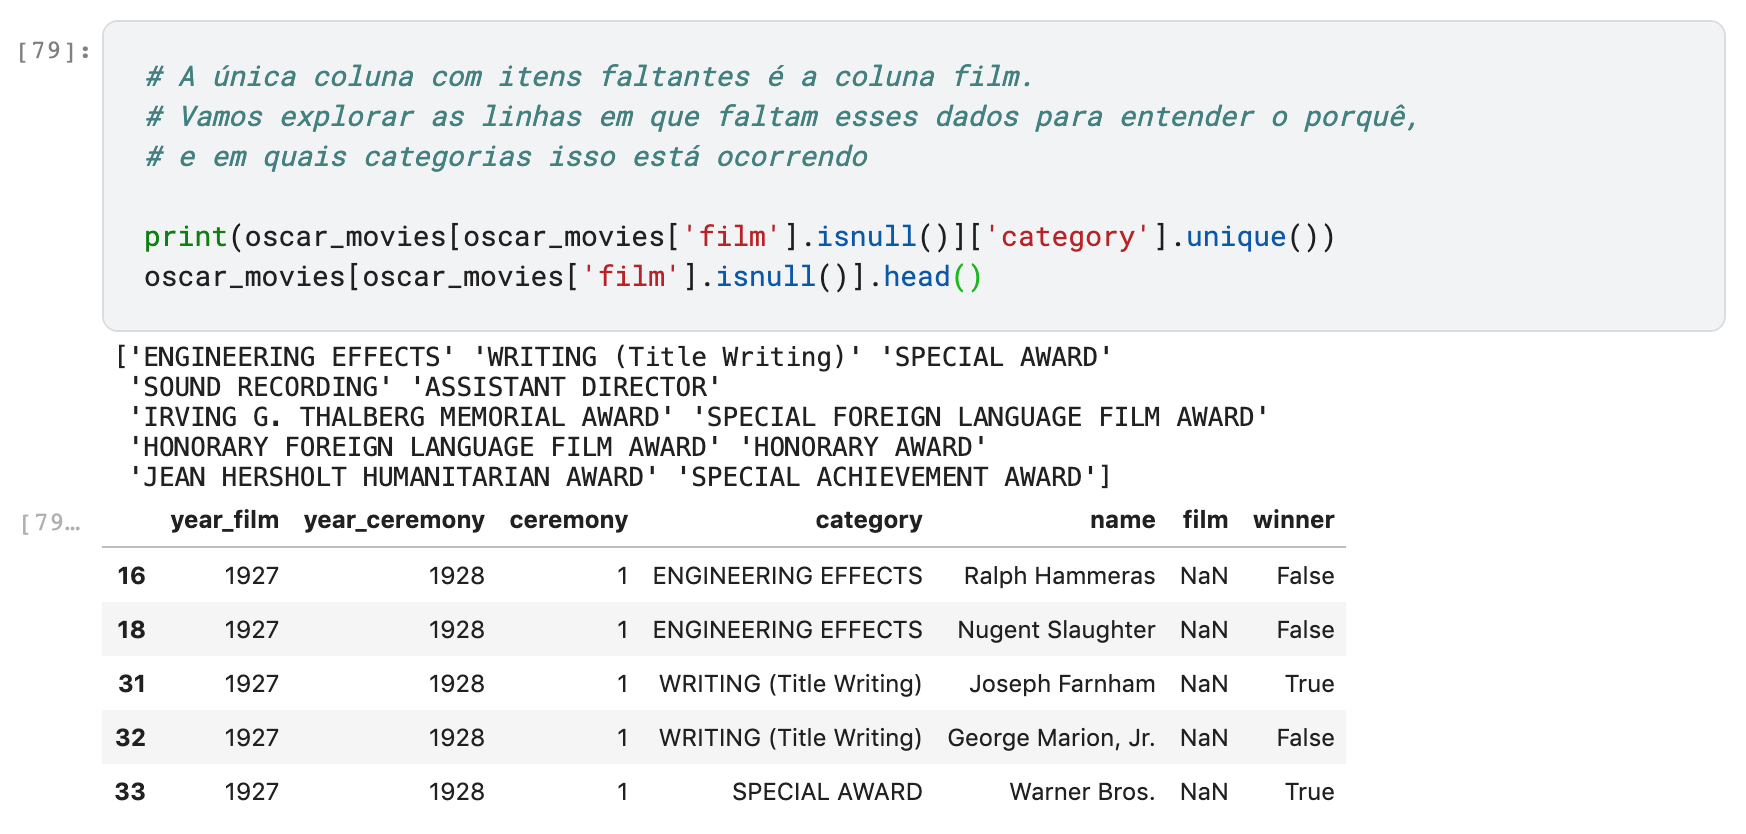
\includegraphics[scale=0.5]{faltantes_film.png}
            	\end{center}
            	\legend{Fonte: trabalho nosso}
            \end{figure}

            Em algumas dessas categorias, nota-se que se trata de prêmios honorários, humanitários ou de conjunto da obra. Esses dados foram desconsiderados, já que não se referem a um filme específico.

            Já para duas das categorias que apresentam dados faltantes - "SPECIAL FOREIGN LANGUAGE FILM AWARD"
            e "HONORARY FOREIGN LANGUAGE FILM AWARD" -, é possível perceber que o nome se encontra na coluna 'name', precisando apenas de tratamento em alguns casos, podendo então ser transferido para a coluna "film".

            Outras linhas com dados faltantes na coluna 'film' são de obtenção difícil ou imprecisa: um assistente de direção, por exemplo, pode ter tido mais de um filme lançado num mesmo ano, o que faria a checagem dos dados restantes muito trabalhosa. Essas colunas serão ignoradas, nos deixando ao final com 10098 linhas completas no dataset.

            Um fato que pode ser observado analisando-se esses dados restantes é que algumas das categorias tiveram mudanças de nomes - como foi o caso na premiação de filme de língua estrangeira. Já outras categorias desapareceram da premiação ("melhor filme em preto e branco") ou foram incluídas. A categoria mais recente incluída na premiação é a de melhor filme de animação, criada em 2002. \cite{usatoday2002}.

            Por esse fator, iremos desconsiderar filmes anteriores a essa data. Essa abordagem tem ainda a vantade de delimitar um recorte cronológico mais coeso, permitindo a visualisação de tendências, o que seria improvável na análise total de quase 100 anos de premiação. Iremos desconsiderar ainda a premiação de edição de som (sound editing), que foi descontinuada em 2019, a única removida após o ano de 2002.\cite{deadline2020}

            Algumas dessas categorias também precisaram de consolidação, já que seus nomes apareciam de formas diferentes. Foram utilizados os nomes mais recentes.

            O passo seguinte é integrar os esquemas dos dois datasets. Para isso, vamos considerar que um filme é o mesmo nos dois datasets caso seu nome e ano apresentem correspondência. Para a análise de nome, serão observadas as colunas 'title' (em alguns casos, também a 'original\_title') do dataset de metadados, e a coluna 'film' do dataset do Oscar.

            Para análise dos anos, foi criada no dataset de metadados uma coluna 'release\_year', extraindo o ano da coluna 'release\_date'. Esse valor será comparado com a coluna 'year\_film' do dataset do Oscar.

            Mas para fazer essa união entre as duas tabelas, foi também necessário normalizar nomes nas duas tabelas, adicionando-se as colunas "normalized\_title" e "normalized\_original\_title". Alguns dos desafios encontrados nesse estágio foram:

            \begin{itemize}
                \item remoção de caracteres especiais e capitalização;
                \item existência, na tabela do Oscar, de filmes com título em inglês ou no original em outra língua;
                \item títulos estilizados (geralmente com pontuação no nome);
                \item filmes com anos diferentes nos dois datasets.
            \end{itemize}

            Esse último item diz respeito à observação de filmes com ano de lançamento ('release\_year') diferentes do ano na tabela do Oscar (coluna 'year\_film'). Um exemplo é o filme 'Y tu mamá también', cuja coluna 'year\_film' tem valor 2002 no dataset do Oscar e 2001 no dataset de metadados. Foram observadas desigualdades entre os anos de até 2 anos, fato que pode estar relacionado à confusão entre as datas de produção e lançamento de um filme. Nesses casos, a coluna 'year\_film' será corrigida para o valor presente na tabela de metadados.


            Com essas informações, já é possível relacionar entre as tabelas 763 dos 942 filmes existentes no dataset do Oscar. Para os restantes 179 filmes, dois desafios especiais se deram:\par

            \begin{itemize}
                \item títulos em inglês diferentes de acordo com o país - por exemplo, o filme "Harry Potter e a Pedra Filosofal", lançado nos Estados Unidos e Índia como "Harry Potter and the Sorcerer's Stone" e nos outros países de língua inglesa "Harry Potter and the Philosopher's Stone"; \cite{yahoo2000};\par
                \item títulos divergentes entre as duas tabelas (como "Mt. Head" na tabela do Oscar, que consta como "Mount head" na tabela de metadados de filmes).\par
            \end{itemize}

            Para esses casos, foi realizada uma análise de similaridade entre os títulos não encontrados nas duas tabelas, utilizando a biblioteca nativa difflib do Python, e uma análise caso a caso.

            Nessa análise, foram encontradas outras 11 correspondências, que tiveram seus anos e nomes ajustados na tabela do Oscar. São os títulos abaixo:\newline

            \begin{figure}[htb]
            	\caption{\label{corresp}Correspondências inexatas encontradas}
            	\begin{center}
            		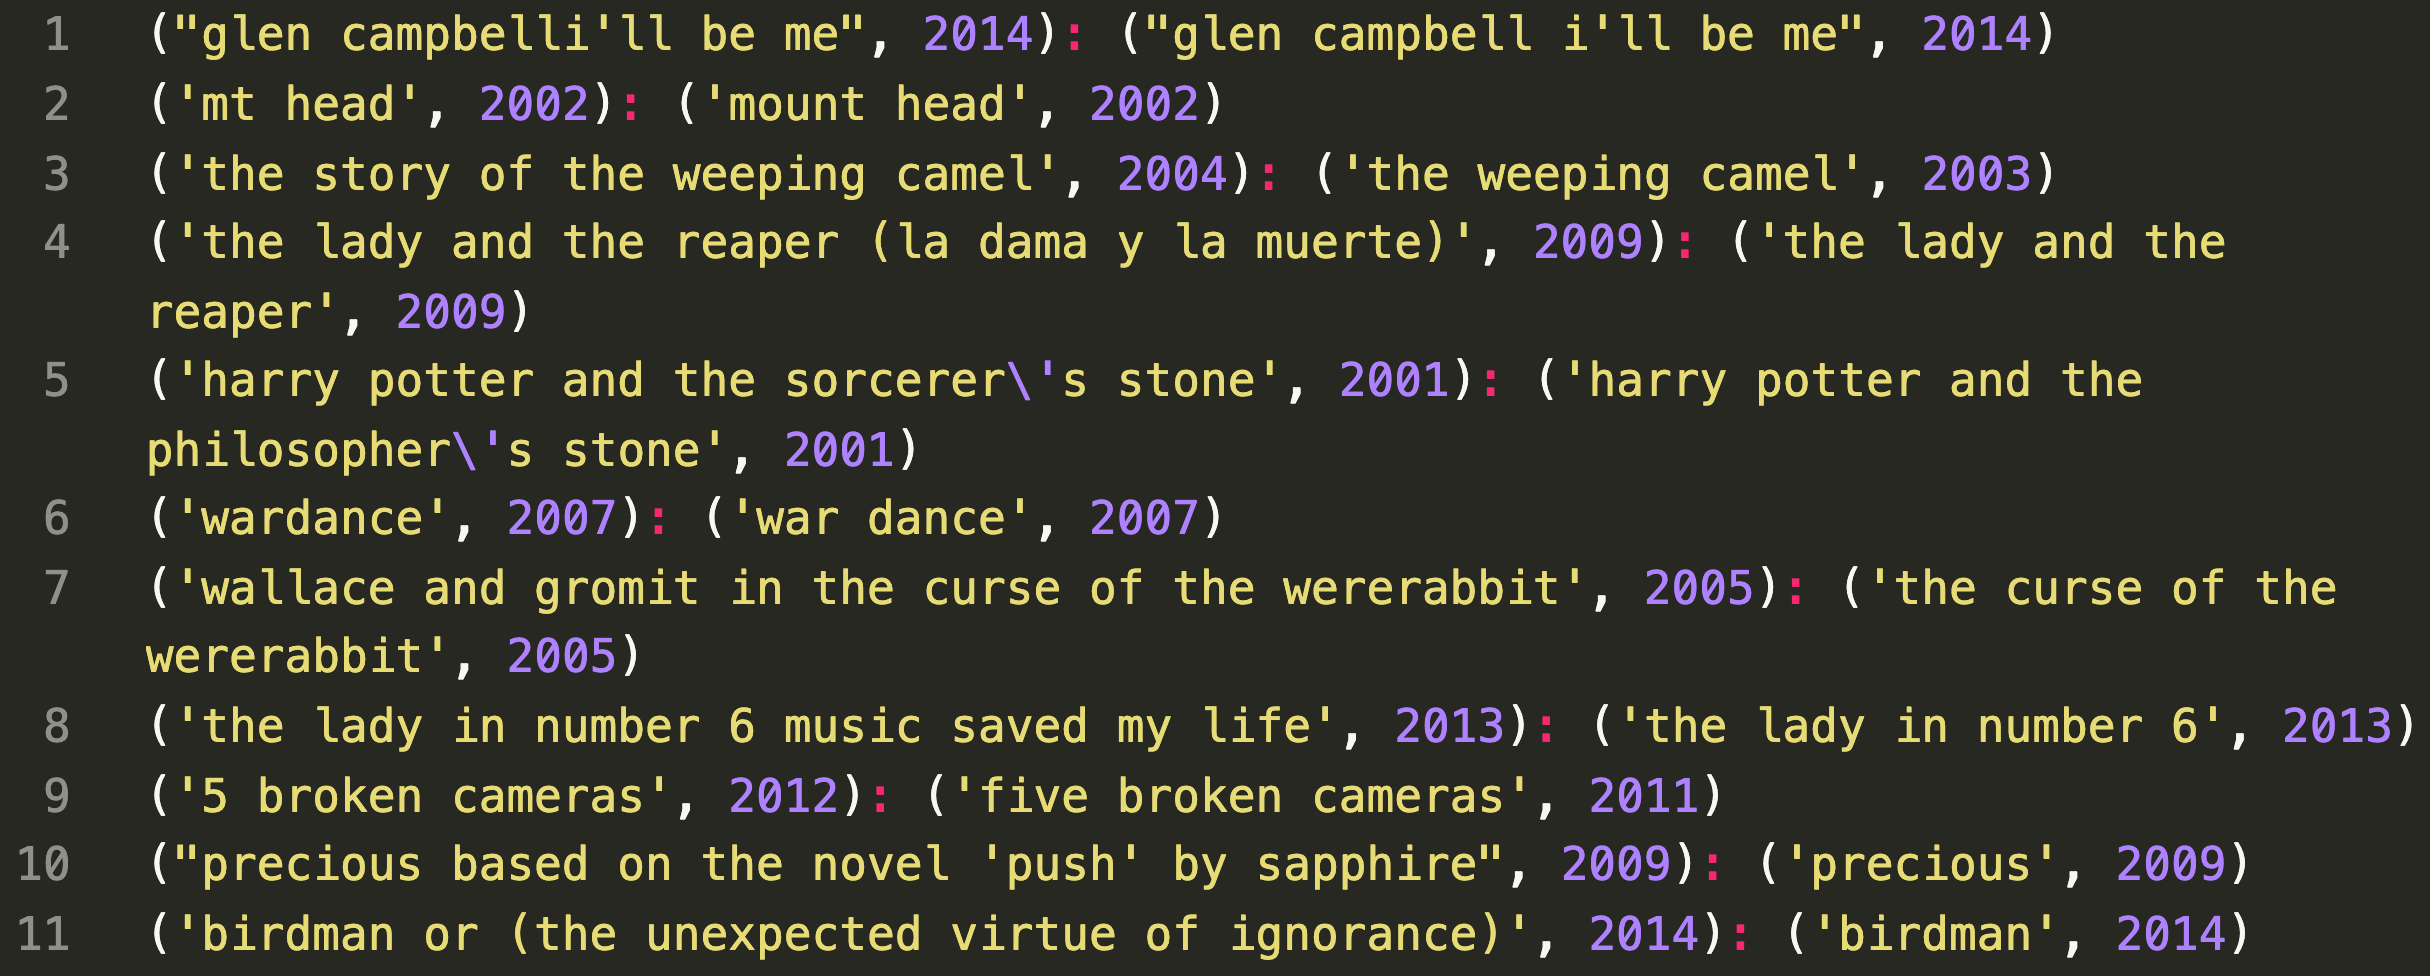
\includegraphics[scale=0.35]{corresp.png}
            	\end{center}
            	\legend{Fonte: trabalho nosso}
            \end{figure}

            Após essa normalização e integração de instâncias, conseguimos localizar na tabela de metadados 774 dos 942 filmes do Oscar. As informações dos demais 168 serão ignoradas.

            Podemos finalmente adicionar as informações dos Oscars ao The Movies Dataset. Para isso, vamos criar colunas no formato one-hot encoding para inserir as informações de nomeação e vitória em cada categoria para cada filme, seguindo a codificação da figura \ref{cat_cods}.

            \begin{figure}[htb]
            	\caption{\label{cat_cods}Codificação das categorias}
            	\begin{center}
            		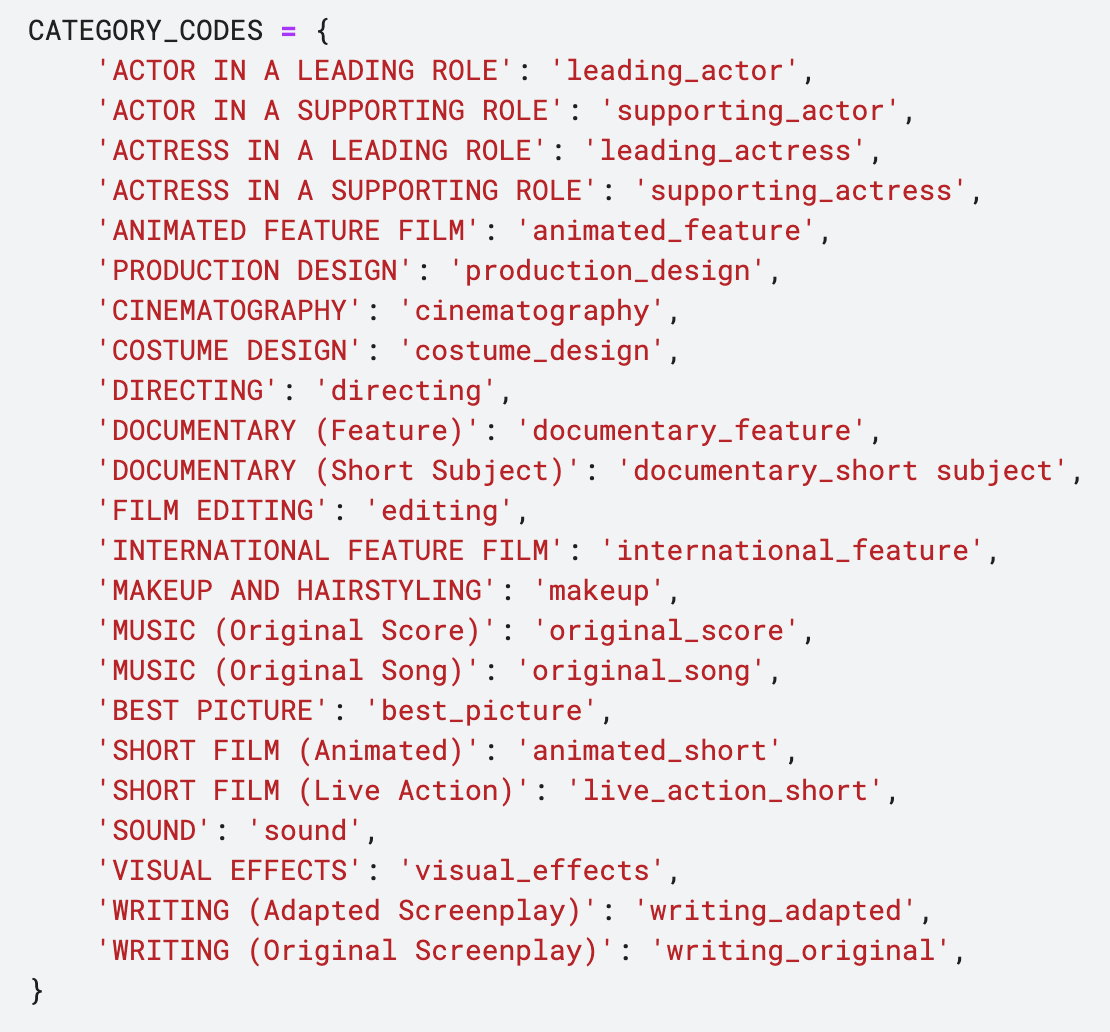
\includegraphics[scale=0.7]{categ_codes.png}
            	\end{center}
            	\legend{Fonte: trabalho nosso}
            \end{figure}

            Para cada um desses códigos, foram criadas duas colunas: '{codigo}\_nominated' e '{codigo}\_won', para designar indicação e vitória na categoria. Também foi adicionada uma coluna para indicar o ano da cerimônia em que participou o filme, com valor None como padrão.\newline

            Após unificados os dados, pôde ser realizada análise exploratória com Pandas, Numpy, e Scikit Learn para conferir a natureza dos dados, a existência de dados faltantes ou inconsistentes e a existência de tendências que auxiliem na construção dos modelos.\newline

            Algumas das colunas analisadas não foram consideradas relevantes na análise, ou quantificáveis. A saber:

            \begin{itemize}
                \item 'belongs\_to\_collection', uma representação da coleção a que supostamente pertence o filme - esse dado está representado de forma bastante subjetiva no dataset;
                \item 'homepage': link para a página oficial do filme;
                \item 'imdb\_id': identificador do filme na plataforma IMDB;
                \item 'original\_title': título original do filme;
                \item 'overview': descrição da trama;
                \item 'poster\_path': url do poster do filme;
                \item 'tagline': frase curta utilizada na publicidade do filme;
            \end{itemize}

            A coluna 'genres' foi convertida em one-hot encoding, levando-se em consideração apenas gêneros que aparecem mais de uma vez na tabela, a saber: 'animation', 'comedy', 'family', 'adventure', 'fantasy', 'romance', 'drama', 'action', 'crime', 'thriller', 'horror', 'history', 'science\_fiction', 'mystery', 'war', 'foreign', 'music', 'documentary', 'western' e 'tv\_movie'. A coluna original foi removida após esse processo.

            A coluna 'production\_companies' poderia trazer informações interessantes, já que um pequeno número de grandes produtoras detêm a maior parte das indicações e premiações\cite{argon2020}. No entanto, uma análise por one-hot encoding seria difícil nesse caso, já que mais de 22900 produtoras foram encontradas na coluna. Por conta disso, optou-se por remover também esse atributo.\newline

            \textbf{Arcabouço de análise exploratória}\par
            Como primeiro ponto da análise exploratória dos dados, foram analisadas as correlações entre as colunas do dataframe. Por se tratar de um grande número de atributos - aproximadamente 240, gerando um número de correlações n**2 de aproximadamente 60000 -, foi necessário experimentar valores mínimos arbitrários para as correlações.\par

            Também ignoramos as correlações entre países de produção. Mesmo as altas entre elas não acrescentavam dados à nossa análise. A coluna que indica filmes produzidos nas Antilhas Holandesas (country\_AN), por exemplo, tem correlação perfeita com a coluna que marca filmes produzidos na Polinésia Francesa (country\_FP).\par

            Experimentamos analisar apenas as 10 correlações maiores que 0.5, mas era possível notar que, mesmo na borda inferior da tabela, onde estavam as correlações menores, ainda era possível ver relações muito relevantes (por exemplo, de indicações em categorias técnicas, por meio das colunas 'nominated\_sound', e 'nominated\_editing, que apresentam uma correlação de 0.5021.\par

            \begin{figure}[htb]
            	\caption{\label{corrs0.5}Correlação entre colunas com valor mínimo de 0.5}
            	\begin{center}
            		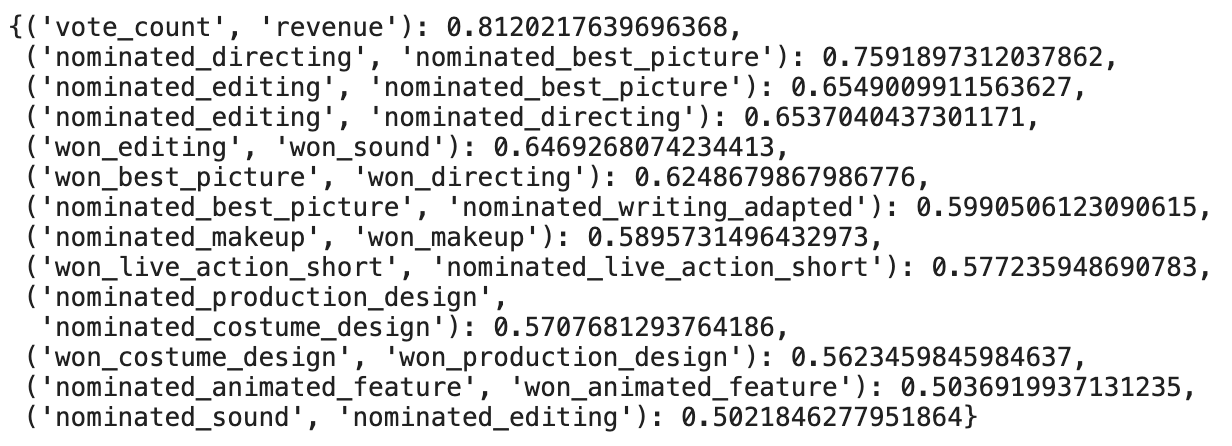
\includegraphics[scale=0.7]{corrs0.5.png}
            	\end{center}
            	\legend{Fonte: trabalho nosso}
            \end{figure}

            Por conta da viabilidade da análise, decidimos nos limitar às 57 correlações maiores do que 0.4. Correlações maiores do que 0.3 já gerariam uma lista com mais de 100 itens (ver figuras \ref{corrs0.5}, \ref{corrs_graph} e \ref{corrs0.4}). \par

            \begin{figure}[htb]
            	\caption{\label{corrs_graph}Número de correlações maiores que cada valor de threshold}
            	\begin{center}
            		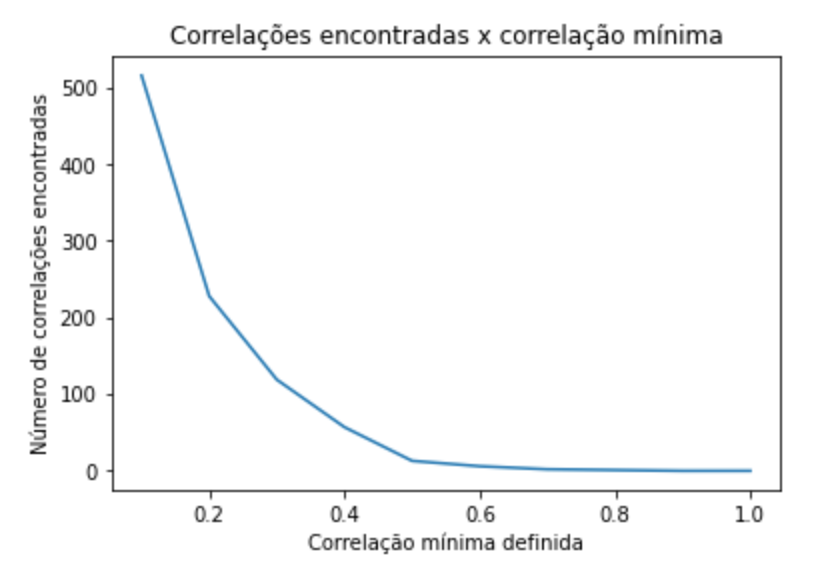
\includegraphics[scale=0.8]{corrs_graph.png}
            	\end{center}
            	\legend{Fonte: trabalho nosso}
            \end{figure}

            \begin{figure}[htb]
            	\caption{\label{corrs0.4}Correlação entre colunas com valor mínimo de 0.4}
            	\begin{center}
            		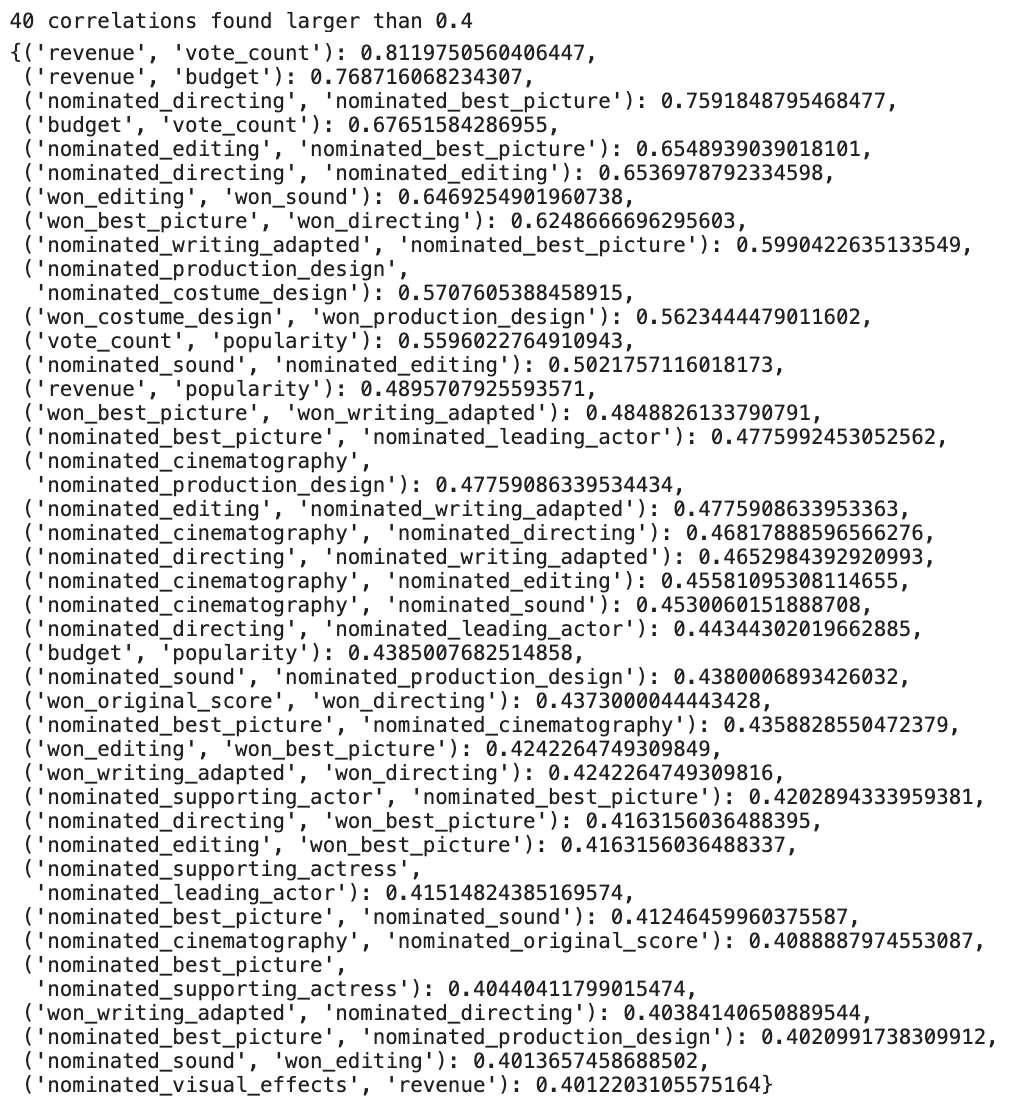
\includegraphics[scale=0.7]{corrs0.4.png}
            	\end{center}
            	\legend{Fonte: trabalho nosso}
            \end{figure}

            Algumas das correlações interessantes reveladas por essa análise, e que podem ajudar na construção dos modelos, ou indicar parâmetros importantes:

            \begin{itemize}
            \item 'vote\_count', o número total de votos que um filme recebeu no site MovieLens tem correlação de 0.81, a mais alta encontrada. Pode indicar que filmes muito assistidos recebem muitos votos no site;
            \item 'vote\_count', o número total de votos que um filme recebeu no site MovieLens tem correlação de 0.81, a mais alta encontrada. Pode indicar que filmes muito assistidos recebem muitos votos no site.
            \end{itemize}

            \textbf{Criação de modelos}\par
            Serão criados modelos de regressão para inferir a chance de premiação utilizando diferentes algoritmos, entre os quais árvores de decisão, regressão logística, support vector machines, random forest e redes neurais.\newline
    
            \textbf{Avaliação comparativa dos resultados}\par
            Avaliação comparativa dos resultados usando as métricas de mean squared error, root mean squared error, e mean absolute error.\newline
    
            \textbf{Avaliação de importância dos metadados}\par
            Avaliação da importância de cada fator (metadado) na previsão, baseando-se no feedback dos algoritmos testados.\newline
    
            \textbf{Interpretação dos resultados}\par
            Interpretação dos resultados para elaboração das conclusões com indicação das técnicas mais promissoras.\newline

        \subsection{Resultados obtidos}

% cola para inserir figura
% \newpage
% \begin{figure}[htb]
% 	\caption{\label{fig_EstruturaTrabAcad}Estrutura do trabalho acadêmico}
% 	\begin{center}
% 		\includegraphics[scale=0.5]{USPSC-EstruturaTrabAcad.jpg}
% 	\end{center}
% 	\legend{Fonte: \citeonline{nbr14724}}
% \end{figure}

% ---

% Capítulo 3 - Desenvolvimento
% ---
% Desenvolvimento
% ---
\chapter[Desenvolvimento]{Desenvolvimento}
% ---
    \section{Considerações iniciais}
    Este capítulo descreve as etapas de desenvolvimento dos modelos de previsão de chances de indicação e premiação no Oscar, detalhando as escolhas realizadas e os procedimentos adotados no processo.

    \section{Atividades realizadas}

        \subsection{Obtenção dos dados}\par

        Foi escolhida como fonte de dados para o trabalho a database "The Movies Dataset", da plataforma Kaggle. Trata-se de um conjunto incluindo metadados para todos os 45.000 filmes listados no conjunto Full MovieLens. O conjunto de dados consiste em filmes lançados em ou antes de julho de 2017. Os dados incluem elenco, equipe, palavras-chave do enredo, orçamento, receita, pôsteres, datas de lançamento, idiomas, empresas de produção, países, contagens de votos TMDB e média de votos".\cite{kaggle2017}\par

        A base de dados 'The Oscar Award, 1927 - 2020' foi utilizada para complementar os metadados, adicionando a eles as informações de indicações na premiação.\cite{kaggle2019}

        \subsection{Limpeza e tratamento dos dados}\par
        
        \begin{figure}[htb]
        	\caption{\label{faltantes_film}Dados faltantes na coluna film}
        	\begin{center}
        		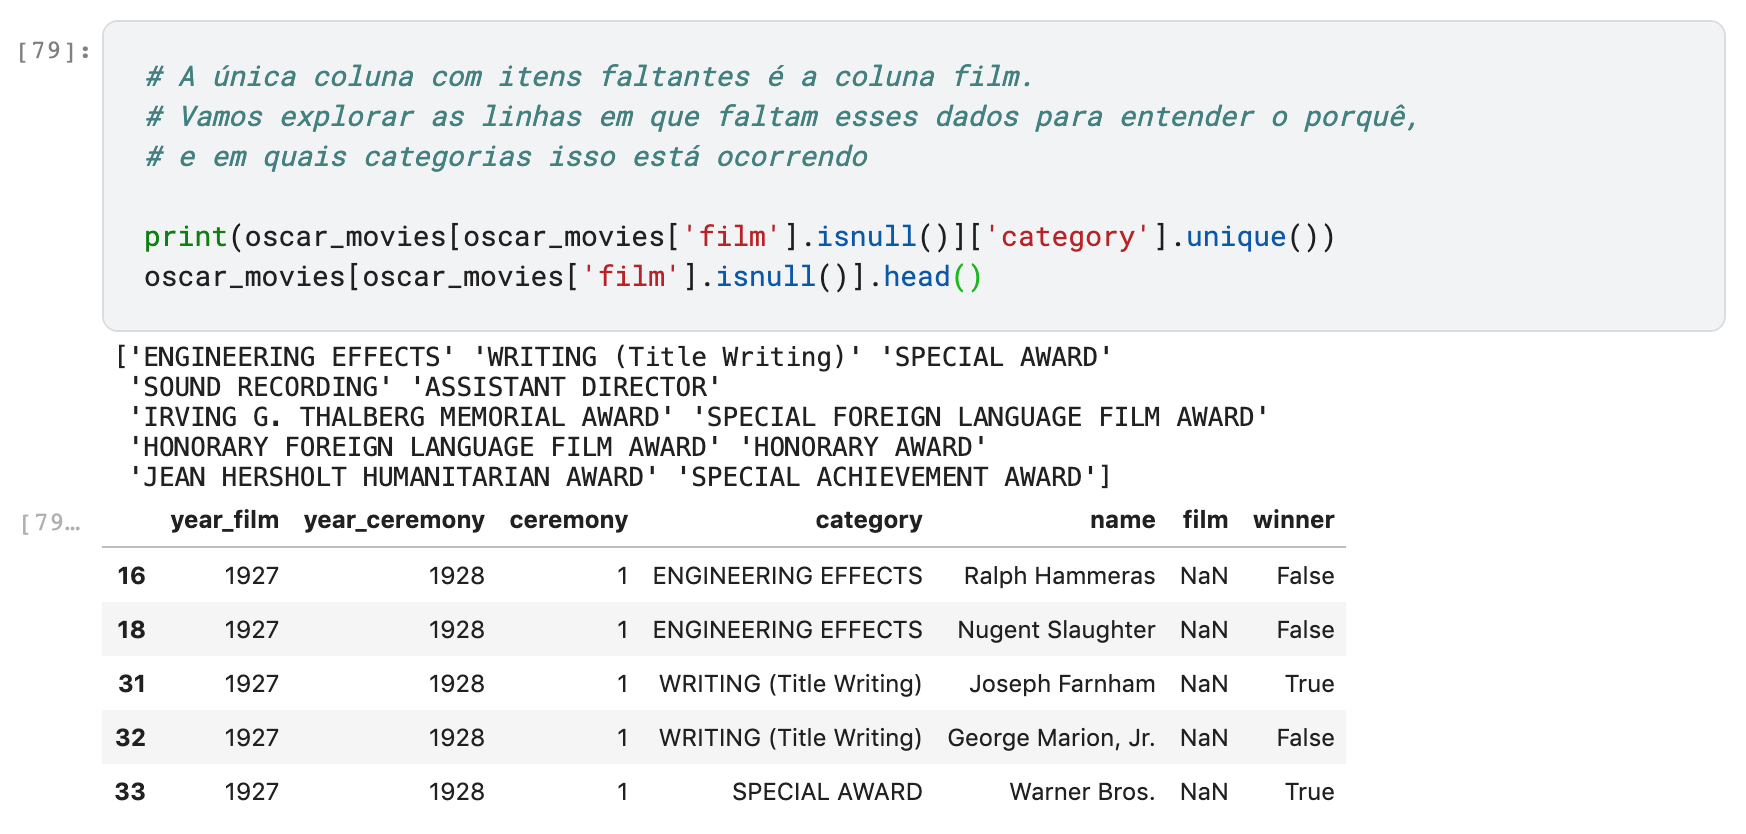
\includegraphics[scale=0.5]{faltantes_film.png}
        	\end{center}
        	\legend{Fonte: trabalho nosso}
        \end{figure}

        O primeiro desafio relacionado à limpeza e tratamento dos dados aparece na base \citeonline{kaggle2019}. Embora a base esteja bastante completa em todas os outras colunas, a coluna 'film' - justamente a que traz o nome do filme relacionado àquela premiação - está nula em 304 linhas  (figura \ref{faltantes_film}).

        Em algumas dessas categorias, nota-se que se trata de prêmios honorários, humanitários ou de conjunto da obra. Esses dados foram desconsiderados, já que não se referem a um filme específico.

        Já para duas das categorias que apresentam dados faltantes - "SPECIAL FOREIGN LANGUAGE FILM AWARD"
        e "HONORARY FOREIGN LANGUAGE FILM AWARD" -, é possível perceber que o nome se encontra na coluna 'name', precisando apenas de tratamento em alguns casos, podendo então ser transferido para a coluna "film".

        Outras linhas com dados faltantes na coluna 'film' são de obtenção difícil ou imprecisa: um assistente de direção, por exemplo, pode ter tido mais de um filme lançado num mesmo ano, o que faria a checagem dos dados restantes muito trabalhosa. Essas colunas serão ignoradas, nos deixando ao final com 10098 linhas completas no dataset.

        Um fato que pode ser observado analisando-se esses dados restantes é que algumas das categorias tiveram mudanças de nomes - como foi o caso na premiação de filme de língua estrangeira. Já outras categorias desapareceram da premiação ("melhor filme em preto e branco") ou foram incluídas. A categoria mais recente incluída na premiação é a de melhor filme de animação, criada em 2002. \cite{usatoday2002}.

        Por esse fator, iremos desconsiderar filmes anteriores a essa data. Essa abordagem tem ainda a vantade de delimitar um recorte cronológico mais coeso, permitindo a visualisação de tendências, o que seria improvável na análise total de quase 100 anos de premiação. Iremos desconsiderar ainda a premiação de edição de som (sound editing), que foi descontinuada em 2019, a única removida após o ano de 2002.\cite{deadline2020}

        Algumas dessas categorias também precisaram de consolidação, já que seus nomes apareciam de formas diferentes. Foram utilizados os nomes mais recentes.

        O passo seguinte é integrar os esquemas dos dois datasets. Para isso, vamos considerar que um filme é o mesmo nos dois datasets caso seu nome e ano apresentem correspondência. Para a análise de nome, serão observadas as colunas 'title' (em alguns casos, também a 'original\_title') do dataset de metadados, e a coluna 'film' do dataset do Oscar. 

        Para análise dos anos, foi criada no dataset de metadados uma coluna 'release\_year', extraindo o ano da coluna 'release\_date'. Esse valor será comparado com a coluna 'year\_film' do dataset do Oscar.
        
        A coluna release\_date também será eliminada em favor de uma coluna com um valor inteiro: release\_day, o número de dias desde o começo do ano até o dia em que o filme foi lançado (indo de 1 a 366). O motivo dessa transformação é a percepção comum de que filmes lançados perto do final do ano têm maiores chances de serem indicação às premiações \cite{hdsr2020}. 

        Mas para fazer essa união entre as duas tabelas, foi também necessário normalizar nomes nas duas tabelas, adicionando-se as colunas "normalized\_title" e "normalized\_original\_title". Alguns dos desafios encontrados nesse estágio foram:

        \begin{itemize}
            \item remoção de caracteres especiais e capitalização;
            \item existência, na tabela do Oscar, de filmes com título em inglês ou no original em outra língua;
            \item títulos estilizados (geralmente com pontuação no nome);
            \item filmes com anos diferentes nos dois datasets.
        \end{itemize}

        \begin{figure}[htb]
        	\caption{\label{corresp}Correspondências inexatas encontradas}
        	\begin{center}
        		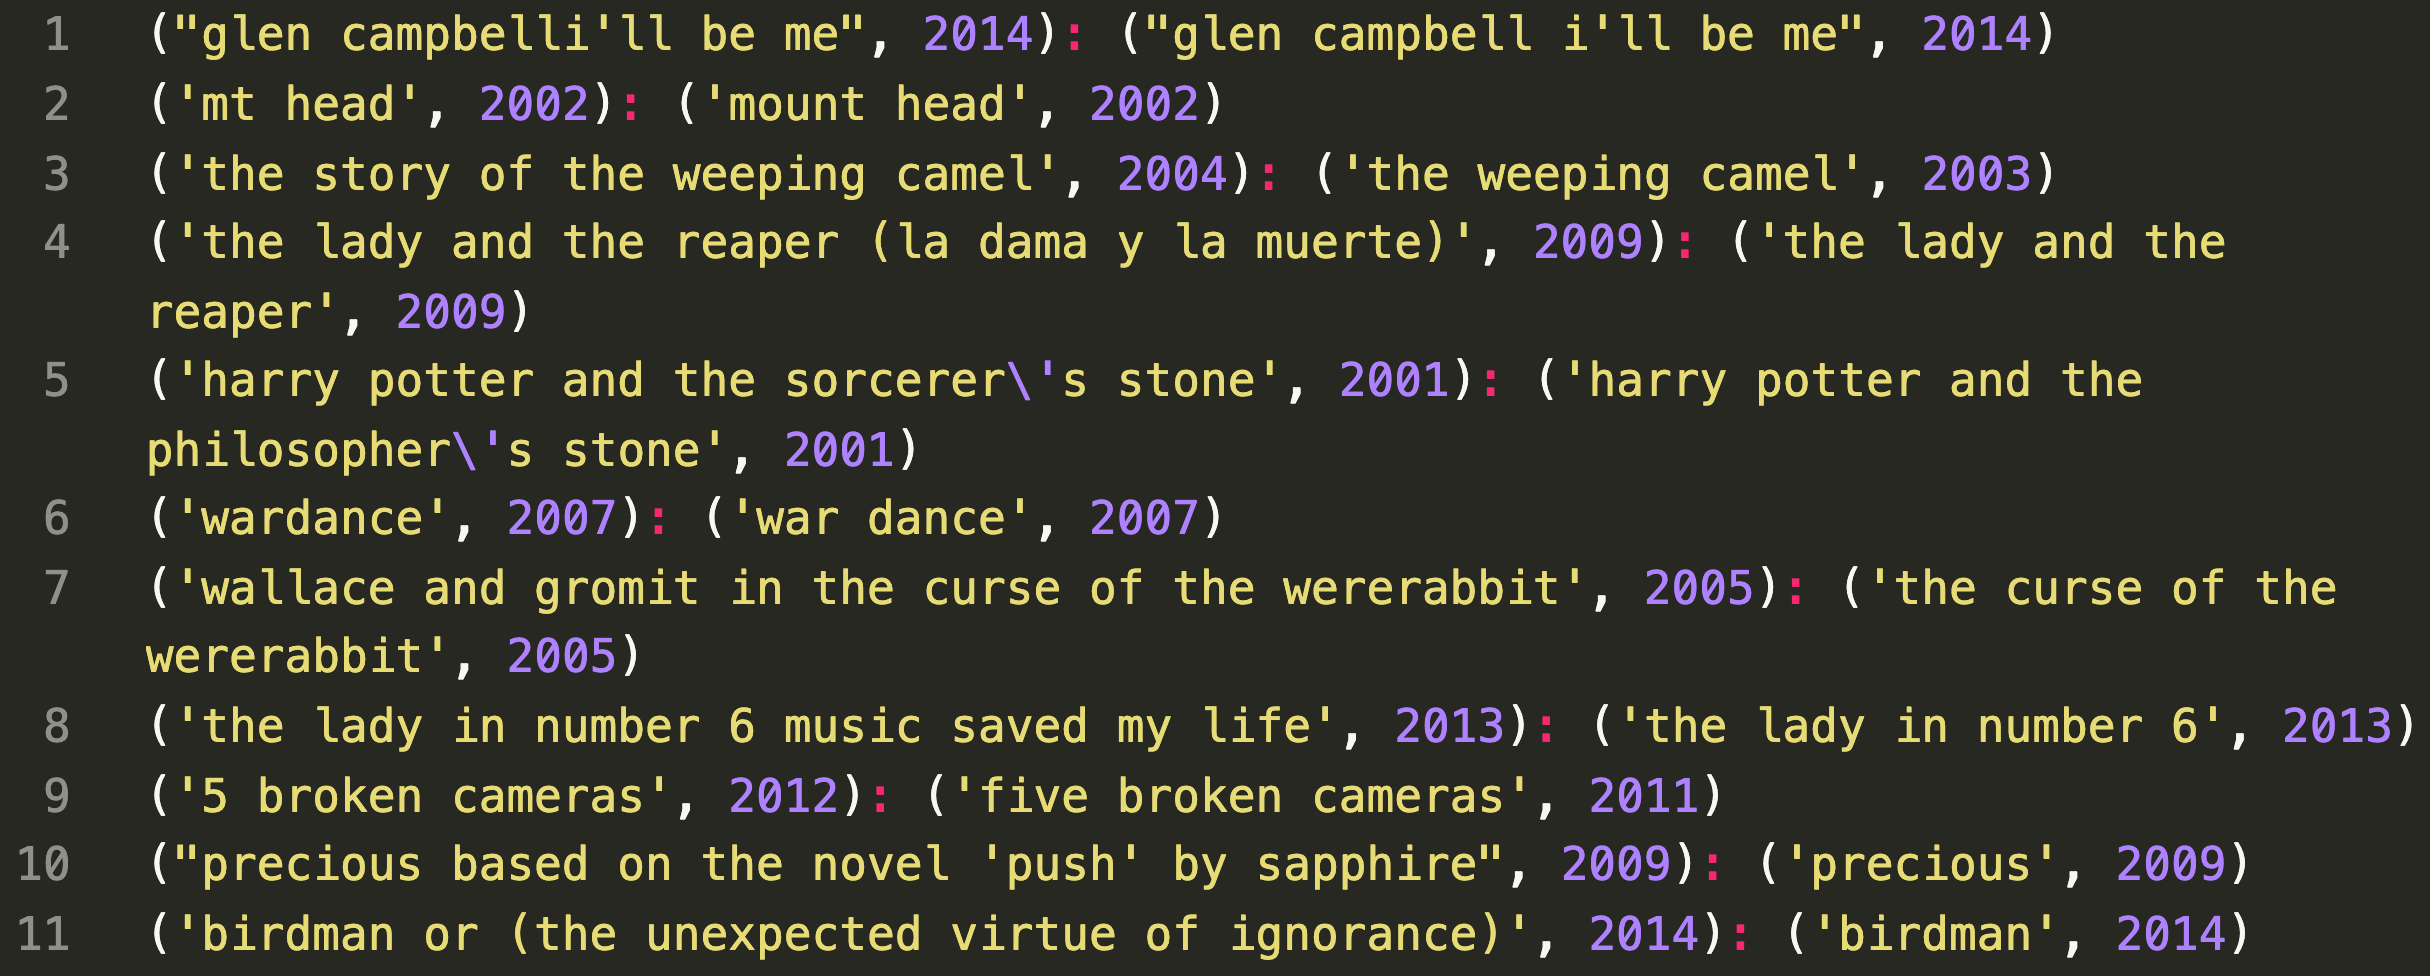
\includegraphics[scale=0.35]{corresp.png}
        	\end{center}
        	\legend{Fonte: trabalho nosso}
        \end{figure}
        
        \begin{figure}[htb]
        	\caption{\label{cat_cods}Codificação das categorias}
        	\begin{center}
        		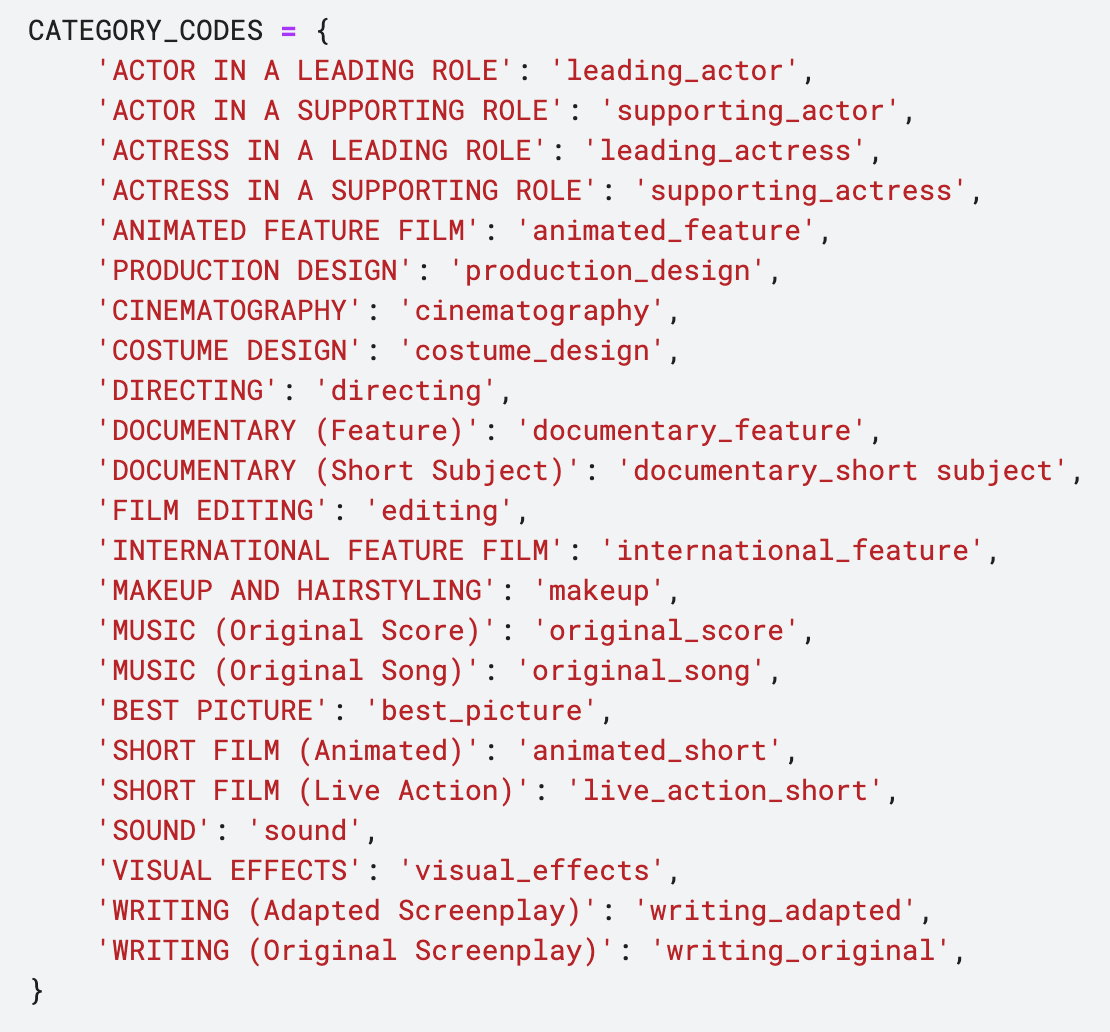
\includegraphics[scale=0.7]{categ_codes.png}
        	\end{center}
        	\legend{Fonte: trabalho nosso}
        \end{figure}

        Esse último item diz respeito à observação de filmes com ano de lançamento ('release\_year') diferentes do ano na tabela do Oscar (coluna 'year\_film'). Um exemplo é o filme 'Y tu mamá también', cuja coluna 'year\_film' tem valor 2002 no dataset do Oscar e 2001 no dataset de metadados. Foram observadas desigualdades entre os anos de até 2 anos, fato que pode estar relacionado à confusão entre as datas de produção e lançamento de um filme. Nesses casos, a coluna 'year\_film' será corrigida para o valor presente na tabela de metadados.


        Com essas informações, já é possível relacionar entre as tabelas 760 dos 942 filmes existentes no dataset do Oscar. Para os restantes 182 filmes, dois desafios especiais se deram:\par

        \begin{itemize}
            \item títulos em inglês diferentes de acordo com o país - por exemplo, o filme "Harry Potter e a Pedra Filosofal", lançado nos Estados Unidos e Índia como "Harry Potter and the Sorcerer's Stone" e nos outros países de língua inglesa "Harry Potter and the Philosopher's Stone"; \cite{yahoo2000};\par
            \item títulos divergentes entre as duas tabelas (como "Mt. Head" na tabela do Oscar, que consta como "Mount head" na tabela de metadados de filmes).\par
        \end{itemize}

        Para esses casos, foi realizada uma análise de similaridade entre os títulos não encontrados nas duas tabelas, utilizando a biblioteca nativa difflib do Python, e uma análise caso a caso.

        Nessa análise, foram encontradas outras 11 correspondências, que tiveram seus anos e nomes ajustados na tabela do Oscar (figura \ref{corresp}).

        Após essa normalização e integração de instâncias, conseguimos localizar na tabela de metadados 771 dos 942 filmes do Oscar. As informações dos demais 168 serão ignoradas.

        Podemos finalmente adicionar as informações dos Oscars ao The Movies Dataset. Para isso, vamos criar colunas no formato one-hot encoding para inserir as informações de nomeação e vitória em cada categoria para cada filme, seguindo a codificação da figura \ref{cat_cods}.

        Para cada um desses códigos, foram criadas duas colunas: '{codigo}\_nominated' e '{codigo}\_won', para designar indicação e vitória na categoria. Também foi adicionada uma coluna para indicar o ano da cerimônia em que participou o filme, com valor None como padrão.

        Após unificados os dados, pôde ser realizada análise exploratória com Pandas, Numpy, e Scikit Learn para conferir a natureza dos dados, a existência de dados faltantes ou inconsistentes e a existência de tendências que auxiliem na construção dos modelos.

        A coluna 'genres' foi convertida em one-hot encoding, resultado nas colunas: 'animation', 'comedy', 'family', 'adventure', 'fantasy', 'romance', 'drama', 'action', 'crime', 'thriller', 'horror', 'history', 'science\_fiction', 'mystery', 'war', 'foreign', 'music', 'documentary', 'western' e 'tv\_movie'.

        O mesmo processo foi aplicado nas colunas country, 'spoken\_languages' e 'original\_language', desconsiderando linguagens e países que aparecem em menos de 500 filmes.

        A coluna 'production\_companies' poderia trazer informações interessantes, já que um pequeno número de grandes produtoras detêm a maior parte das indicações e premiações \cite{argon2020}. No entanto, uma análise por one-hot encoding seria difícil nesse caso, já que mais de 15336 produtoras foram encontradas na coluna. Por conta disso, optou-se por remover também esse atributo.

        Alguns tratamentos pontuais foram realizados para modificar e padronizar os valores de algumns atributos: as colunas 'adult' (que indica se um filme é adulto), 'video' (que aponta lançamentos feitos direto para o video) e 'budget' (orçamento) foram transformadas em float.
        
        Foram localizados também 3 filmes com valores float (NaN) na coluna 'title'. Essas três instâncias parecem ter o mesmo problema: colunas desalinhadas pela falta de algum valor. Na impossibilidade de confirmar exatamente quais dados pertencem a quais colunas, vamos eliminá-las.
        
        Havia também filmes marcados no dataset como especulados, em produção, etc. Como apenas podem ser considerados ao Oscar filmes que efetivamente tenham sido lançados, checamos se algum dos filmes especulados, em produção, etc, recebeu alguma indicação ou prêmio e está com o status errado. Os outros foram descartados.
        
        Ao final do processo, algumas das colunas existentes não foram consideradas relevantes na análise e foram removidas. A saber:

        \begin{itemize}
            \item 'belongs\_to\_collection', uma representação da coleção a que supostamente pertence o filme - esse dado está representado de forma bastante subjetiva no dataset;
            \item 'homepage': link para a página oficial do filme;
            \item 'imdb\_id': identificador do filme na plataforma IMDB;
            \item 'id': identificador do filme na plataforma MovieLens;
            \item 'original\_title': título original do filme;
            \item 'overview': descrição da trama;
            \item 'poster\_path': url do poster do filme;
            \item 'tagline': frase curta utilizada na publicidade do filme;
            \item 'original\_language' (convertida em one-hot encoding)
            \item 'spoken\_languages' (convertida em one-hot encoding)
            \item 'normalized\_title' (utilizada apenas para linkar os dois datasets)
            \item 'normalized\_original\_title' (utilizada apenas para linkar os dois datasets)
            \item 'status' - diz se o filme está em pré-produção, foi finalizado, etc.
        \end{itemize}

        \subsection{Arcabouço de análise exploratória}\par

        \begin{figure}[htb]
        	\caption{\label{corrs_graph}Número de correlações maiores que cada valor de threshold}
        	\begin{center}
        		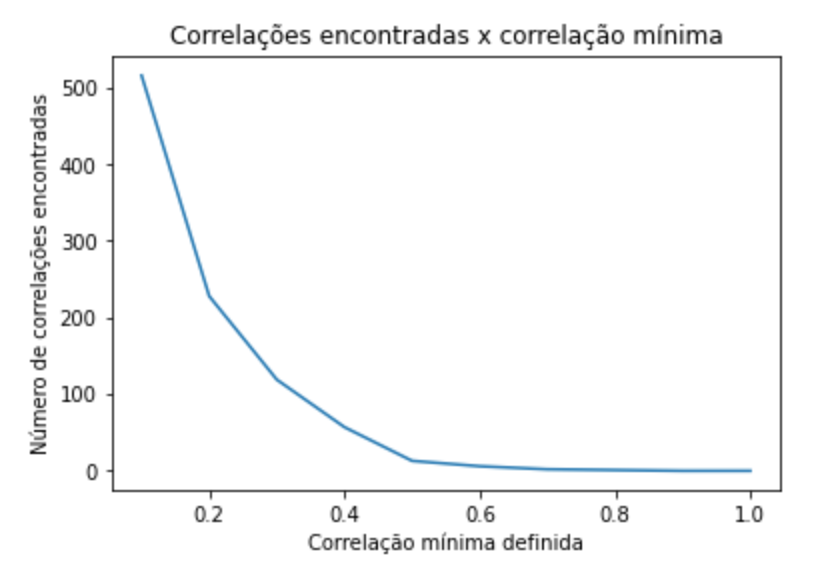
\includegraphics[scale=0.8]{corrs_graph.png}
        	\end{center}
        	\legend{Fonte: trabalho nosso}
        \end{figure}

        % \begin{figure}[htb]
        % 	\caption{\label{corrs0.4}Correlação entre colunas com valor mínimo de 0.4}
        % 	\begin{center}
        % 		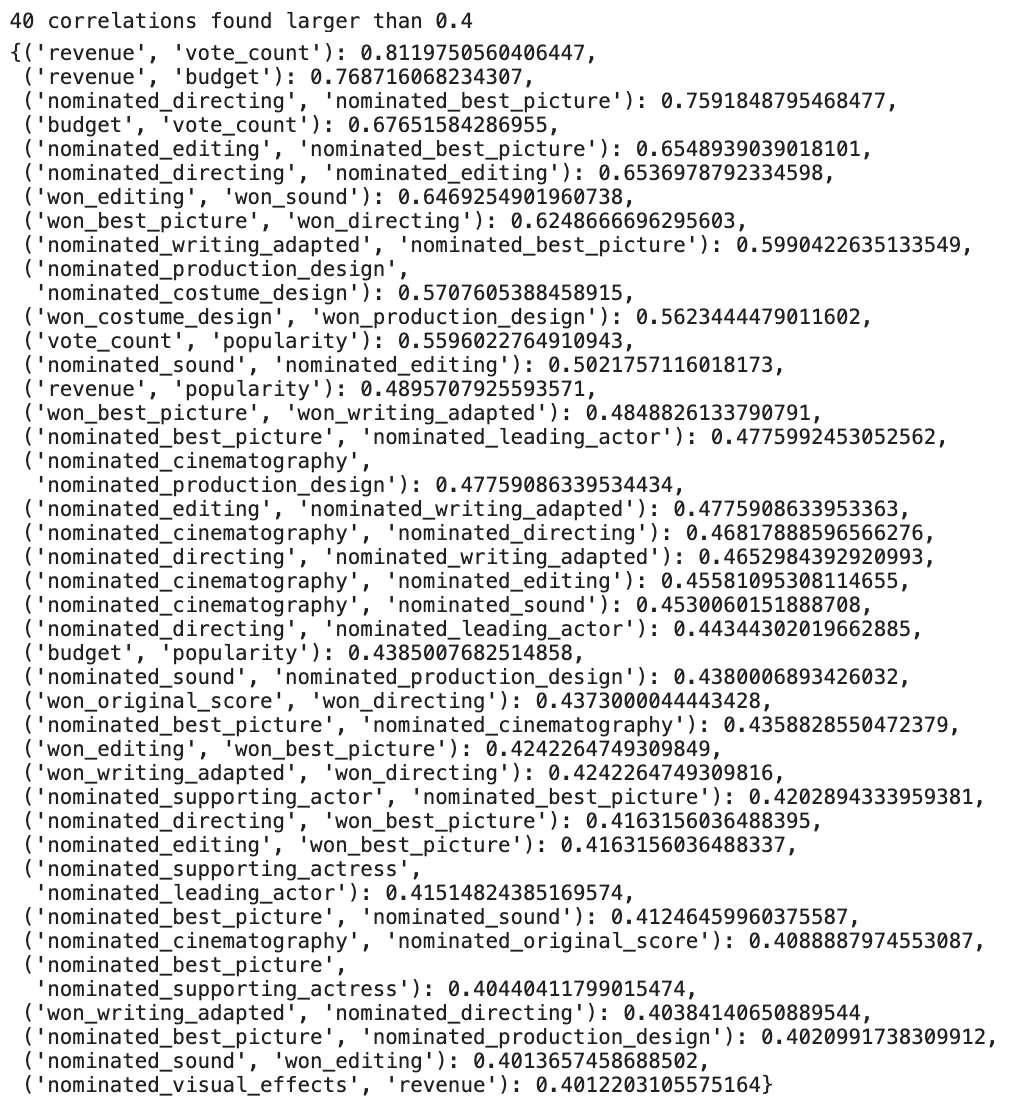
\includegraphics[scale=0.7]{corrs0.4.png}
        % 	\end{center}
        % 	\legend{Fonte: trabalho nosso}
        % \end{figure}

        % \begin{figure}[htb]
        % 	\caption{\label{vencedores_efeitos}Filmes vencedores do Oscar de Efeitos Visuais no dataset analisado}
        % 	\begin{center}
        % 		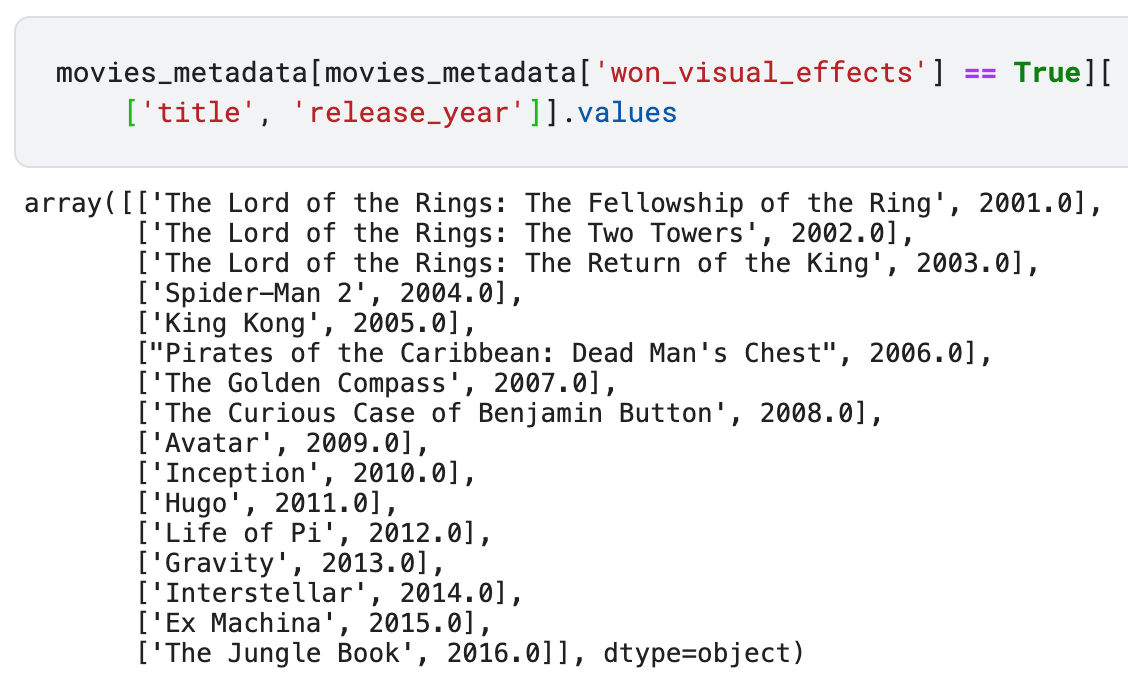
\includegraphics[scale=0.7]{vencedores_efeitos.png}
        % 	\end{center}
        % 	\legend{Fonte: trabalho nosso}
        % \end{figure}

        % \begin{figure}[htb]
        % 	\caption{\label{colunas_influentes_1}Colunas que mais aparecem nas correlações altas (inclui indicações)}
        % 	\begin{center}
        % 		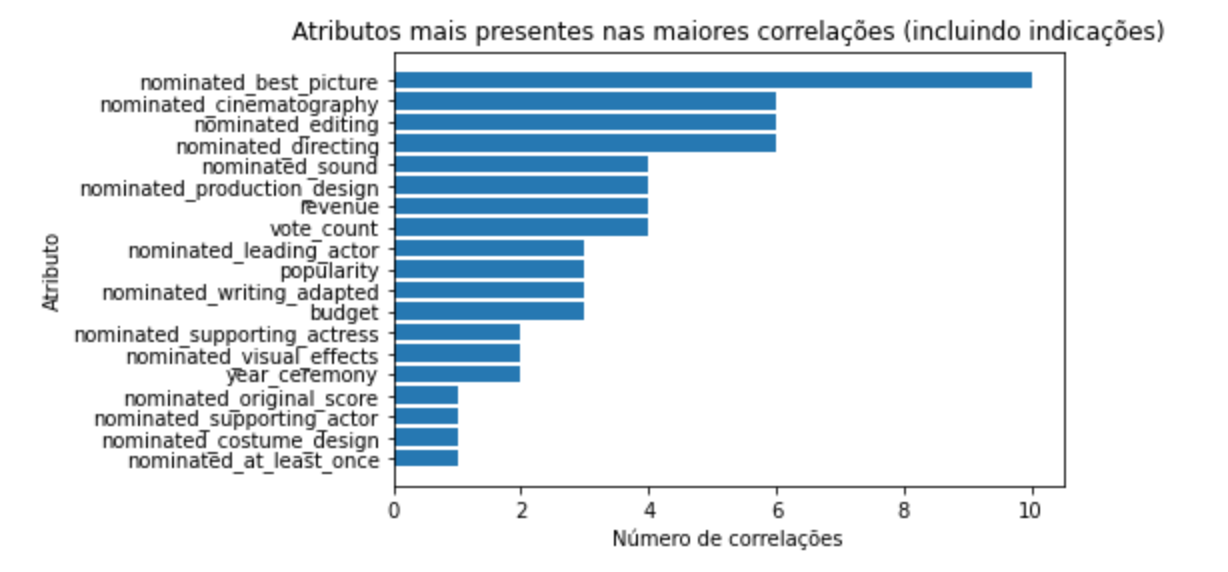
\includegraphics[scale=0.7]{colunas_influentes_1.png}
        % 	\end{center}
        % 	\legend{Fonte: trabalho nosso}
        % \end{figure}

        % \begin{figure}[htb]
        % 	\caption{\label{corrs0.4}Correlação entre colunas com valor mínimo de 0.4 - inclui indicações}
        % 	\begin{center}
        % 		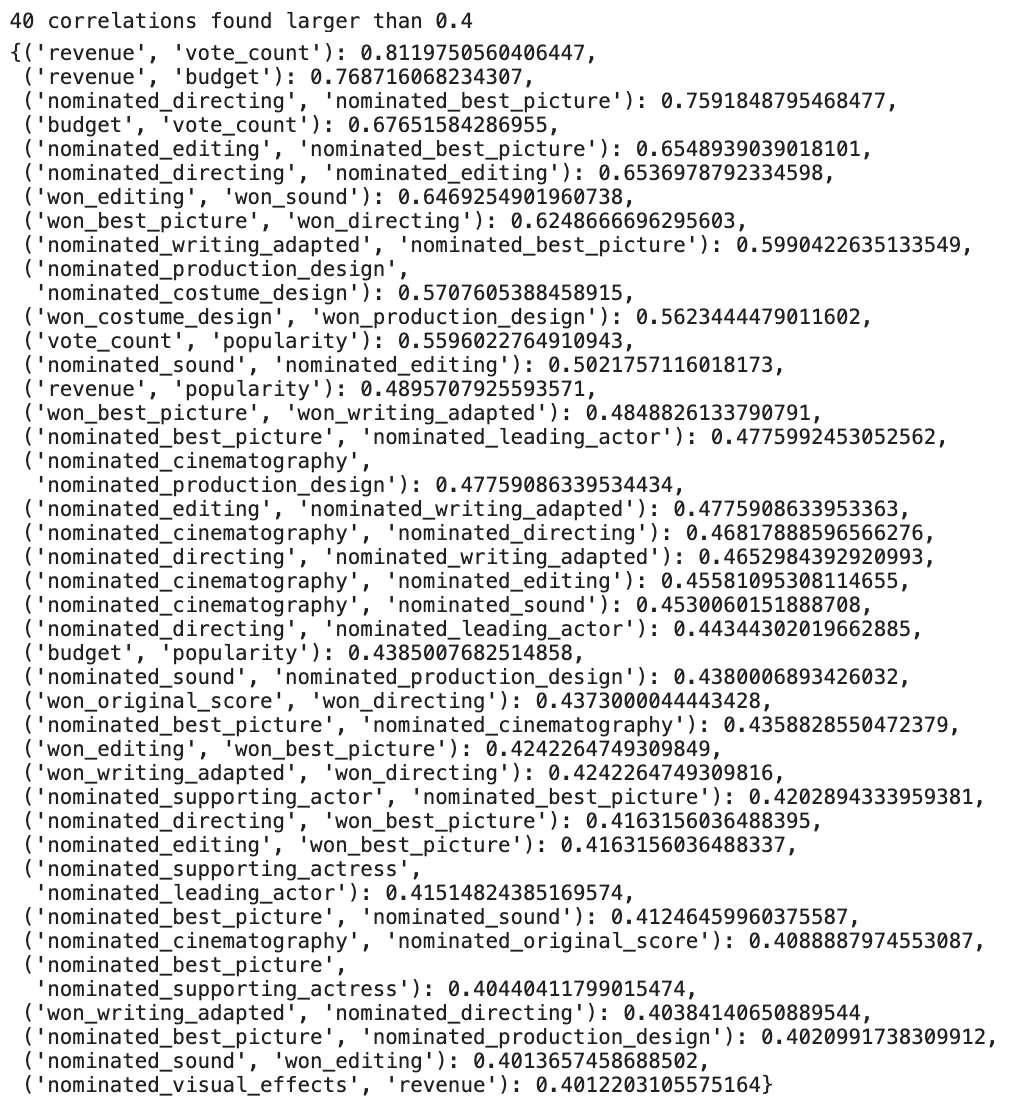
\includegraphics[scale=0.7]{corrs0.4.png}
        % 	\end{center}
        % 	\legend{Fonte: trabalho nosso}
        % \end{figure}
        
        % \begin{figure}[htb]
        % 	\caption{\label{colunas_influentes_2}Colunas que mais aparecem nas correlações altas (inclui indicações)}
        % 	\begin{center}
        % 		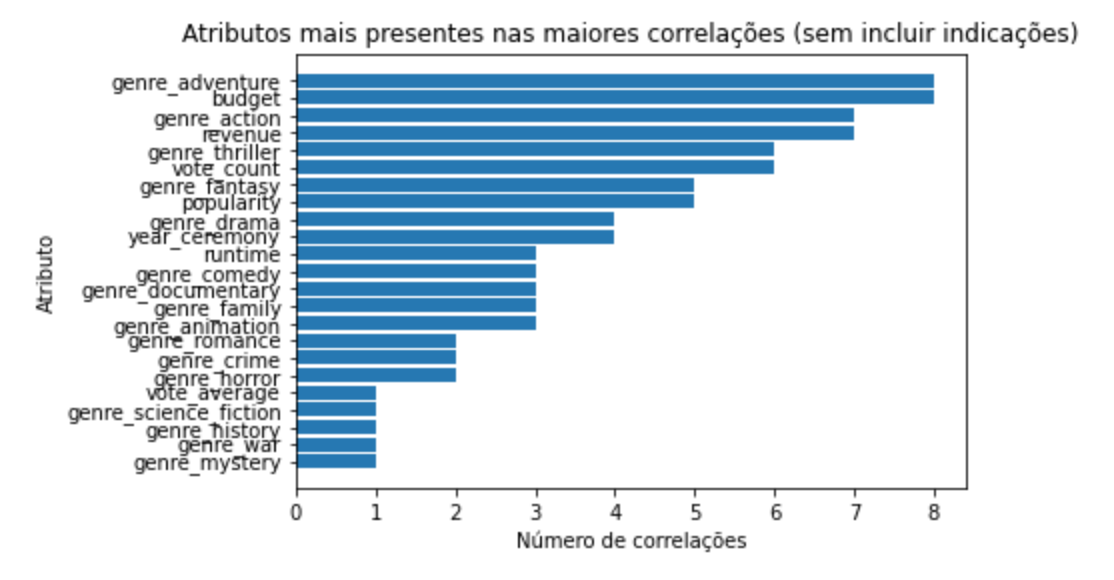
\includegraphics[scale=0.7]{colunas_influentes_2.png}
        % 	\end{center}
        % 	\legend{Fonte: trabalho nosso}
        % \end{figure}

        % \begin{figure}[htb]
        % 	\caption{\label{corrs0.15}Correlação entre colunas com valor mínimo de 0.15 - não inclui indicações}
        % 	\begin{center}
        % 		\includegraphics[scale=0.7]{corrs0.15.png}
        % 	\end{center}
        % 	\legend{Fonte: trabalho nosso}
        % \end{figure}
        
        \begin{figure}[htb]
        	\caption{\label{pca_2}Análise de componente principal em 2 dimensões - vencedores x não-vencedores}
        	\begin{center}
        		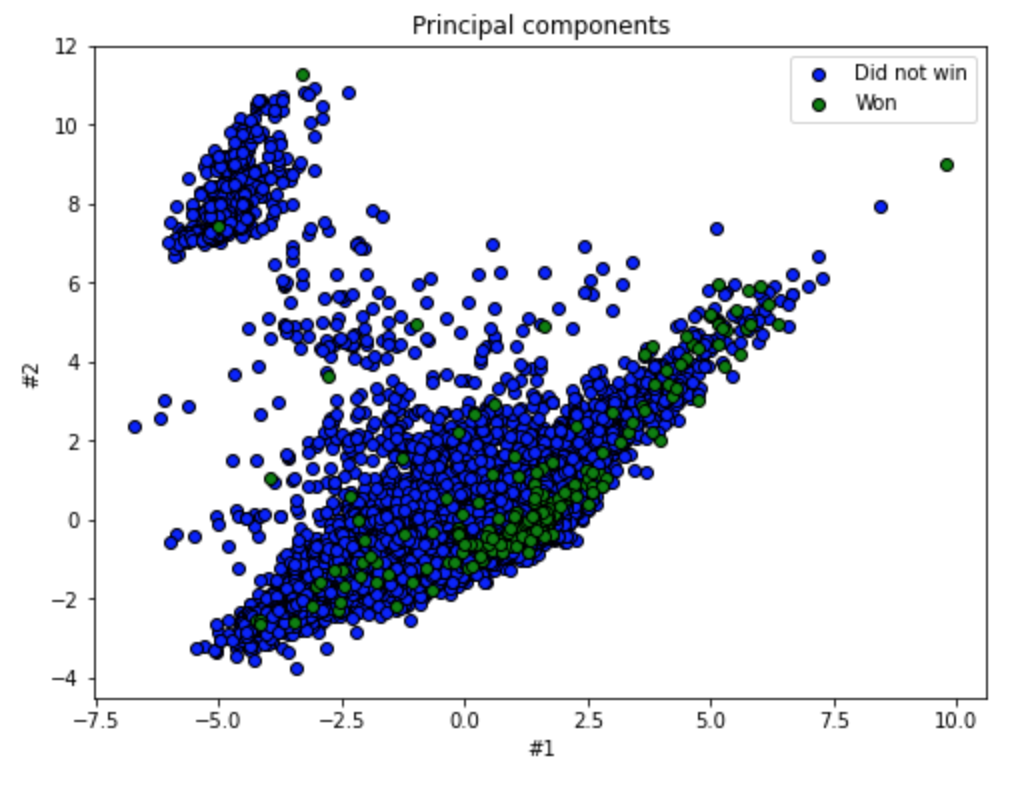
\includegraphics[scale=0.7]{pca_2.png}
        	\end{center}
        	\legend{Fonte: trabalho nosso}
        \end{figure}
        
        % \begin{figure}[htb]
        % 	\caption{\label{pca_3}Análise de componente principal em 3 dimensões - vencedores x não-vencedores}
        % 	\begin{center}
        % 		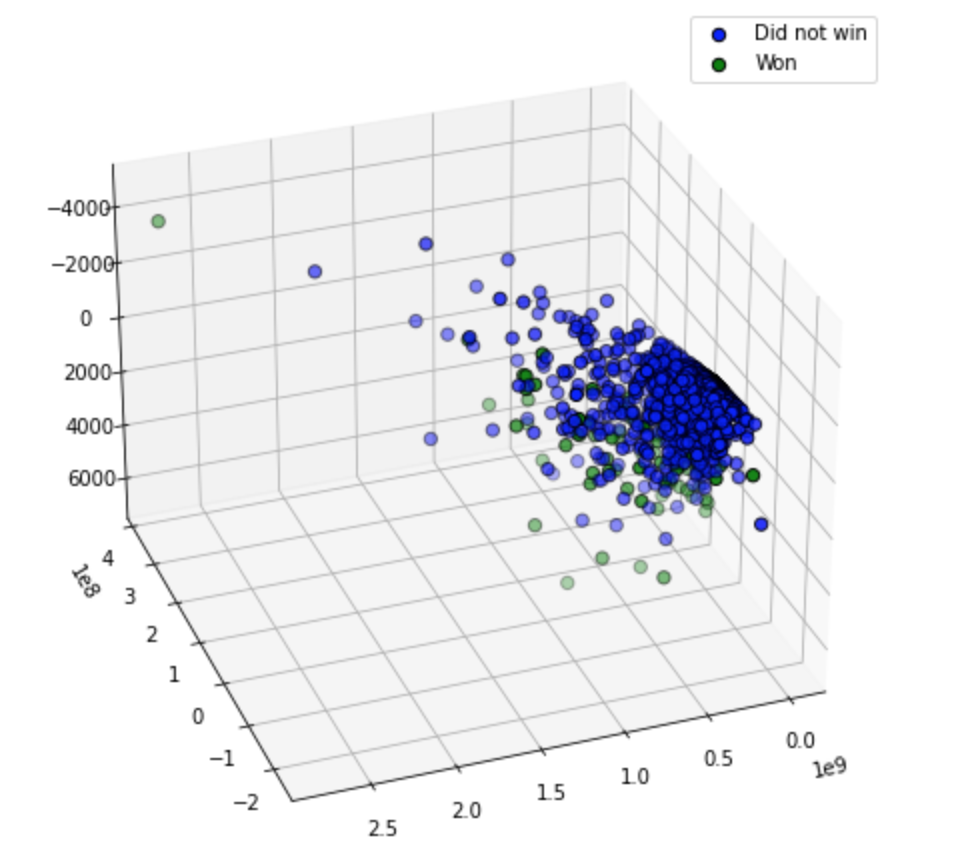
\includegraphics[scale=0.7]{pca_3.png}
        % 	\end{center}
        % 	\legend{Fonte: trabalho nosso}
        % \end{figure}
        
        % \begin{figure}[htb]
        % 	\caption{\label{outliers}Análise de outliers nos atributos numéricos}
        % 	\begin{center}
        % 		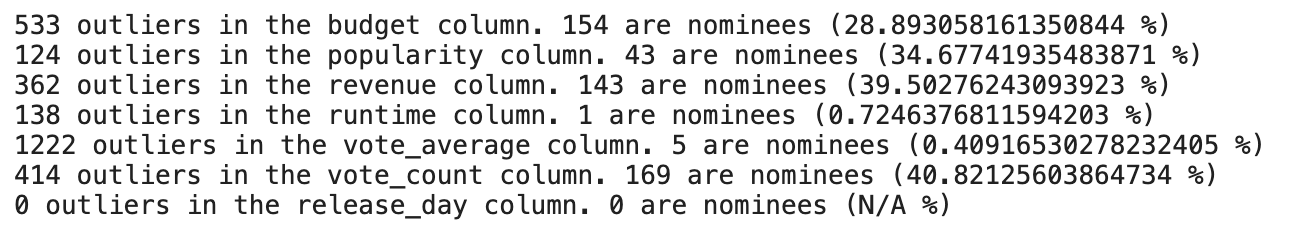
\includegraphics[scale=0.7]{outliers.png}
        % 	\end{center}
        % 	\legend{Fonte: trabalho nosso}
        % \end{figure}

        Como primeiro ponto da análise exploratória dos dados, foram analisadas as correlações entre as colunas do dataframe. Por se tratar de um grande número de atributos - aproximadamente 52, gerando um número de correlações n**2 de aproximadamente 60000 -, foi necessário experimentar valores mínimos arbitrários para as correlações.

        Também ignoramos as correlações entre países de produção. Mesmo as altas entre elas não acrescentavam dados à nossa análise. A coluna que indica filmes produzidos nas Antilhas Holandesas ('country\_AN'), por exemplo, tem correlação perfeita com a coluna que marca filmes produzidos na Polinésia Francesa ('country\_FP').\par

        Levando em conta a viabilidade da análise, decidimos nos limitar às correlações maiores do que 0.4. Correlações maiores do que 0.3 já gerariam uma lista com cerca de 100 itens (figura \ref{corrs_graph}). \par

        Algumas das correlações interessantes reveladas por essa análise, e que podem ajudar na construção dos modelos, ou indicar parâmetros importantes:

        \begin{itemize}

        \item A correlação entre orçamento de um filme e a renda gerada por ele também é muito alta.

        \item Existe grande correlação envolvendo a arrecadação de um filme é a indicação na categoria de efeitos visuais ('nominated\_visual\_effects'). Reforçamos a existência dessa relação entre arrecadação e efeitos visuais ao ver que 12 dos 16 vencedores do oscar de efeitos visuais no nosso dataset final estão na lista de 200 maiores bilheterias da história \cite{mojo2021};

        \item O atributo mais presente nas altas correlações é a coluna 'nominated\_best\_picture'. Há uma grande relação entre filmes indicados ao Oscar de melhor filme, a principal categoria da premiação, e a indicação e vitória em outras categorias.

        \item 10 correlações envolvem as colunas relacionadas ao prêmio de melhor direção ('nominated\_directing' e 'won\_directing').
        
        \end{itemize}
        
        As colunas que representam indicações ('nominated\_*') foram dominantes nessa análise. Mas é preciso levar em consideração que elas serão utilizadas como classe em uma das versões definidas do problema. Por isso, foi feita uma segunda versão da análise, desconsiderando essas colunas, para entender quais são as outras colunas que apresentam grande correlação com os outros atributos.
        
        Nessa versão, para limitar o número de correlações, foram analisadas as correlações superiores a 0.15. Dessa vez, as colunas relativas a gêneros ('genre\_*') foram predominantes.

        Realizamos também projeções, em duas e três dimensões, dos objetos do dataset, utilizando a técnica de Principal Component Analysis (PCA), utilizando cores para representar os filmes vitoriosos ou não.
        
        A representação em duas dimensões mostra um dado interessante: os filmes vitoriosos parecem se concentrar num ponto do espaço, o que pode significa uma maior chance de êxito na criação de superfícies de decisão que tragam uma resposta para o problema (figura \ref{pca_2}).
        
        \subsection{Remoção de outliers}\par
        Foi analisada a possibilidade de remoção de outliers nos atributos numéricos ('budget', 'revenue', 'runtime', e 'release\_day'), considerando-se outliers os valores a mais de 3 desvios-padrão de distância - da média dos atributos.\par
        
        A comparação da proporção de indicados ao Oscar, nossa classe de interesse, entre os outliers em cada um desses atributos mostrou que a remoção de outliers afetaria significativamente a amostragem da classe de interesse, que já é baixa. Por esse motivo, optamos por manter os outliers.

        \subsection{Seleção de atributos}\par
        
        Para permitir a obtenção de melhores resultados, além de reduzir o custo computacional do treinamento dos modelos, foi testada a redução d grande número de atributos do dataset pela regressão por stepwise. Foram utilizados thresholds de inclusão de 0.01 e de exclusão de 0.7, resultando na redução dos 97 atributos para apenas 12: 'revenue', 'release\_day', 'genre\_drama', 'country\_US', 'runtime', 'genre\_history', 'genre\_action', 'spoken\_language\_FR', 'genre\_family', 'original\_language\_EN', 'country\_FR', 'country\_IN'.
        
        Uma segunda versão do modelo foi treinada com atributos selecionados manualmente: 'revenue', 'release\_day', 'genre\_drama', 'country\_US', 'runtime'.

        \subsection{Separação em conjuntos de treinamento, validação e teste}\par
        
        Os dois modelos foram treinados e avaliados seguindo a mesma lógica de separação dos dados: 70\% são usados para treinamento dos modelos; 15\% são utilizados para validar os modelos tentar obter os melhores resultados; e os 15\% finais são guardados para sem utilizados apenas no teste final dos modelos escolhidos.
        
        Para criação desses conjuntos, foi utilizada a função "train\_test\_split" da biblioteca Scikit-learn. A função é aplicada uma vez para separação dos 70\% de treinamento, e uma segunda vez para dividir os 30 \% restantes em conjuntos em teste e validação.\newline
        
        Como os dados possuem classes desbalanceadas (uma fração muito pequena dos filmes é indicada ou vence o Oscar), todas essas operações utilizaram o parametro 'stratify'. Com esse argumento recebendo o valor True, garantimos que todos os subconjuntos criados tenham a mesma proporção de cada positivos e negativos.

        \subsection{Criação de modelos}\par
        Foram criados os seguintes modelos de regressão logística:
        
        \begin{itemize}
            \item Modelo 1: para inferir a chance de indicação na categoria Melhor Filme ("Best Picture"), treinado a partir de atributos selecionados automaticamente pelo método stepwise;
            
            \item Modelo 2: para inferir a chance de indicação na categoria Melhor Filme ("Best Picture"), treinado a partir de atributos selecionados manualmente;

        \end{itemize}
        
        \begin{figure}[htb]
        	\caption{\label{roc1}Curva ROC do modelo de predição de indicação, com seleção stepwise de atributos}
        	\begin{center}
        		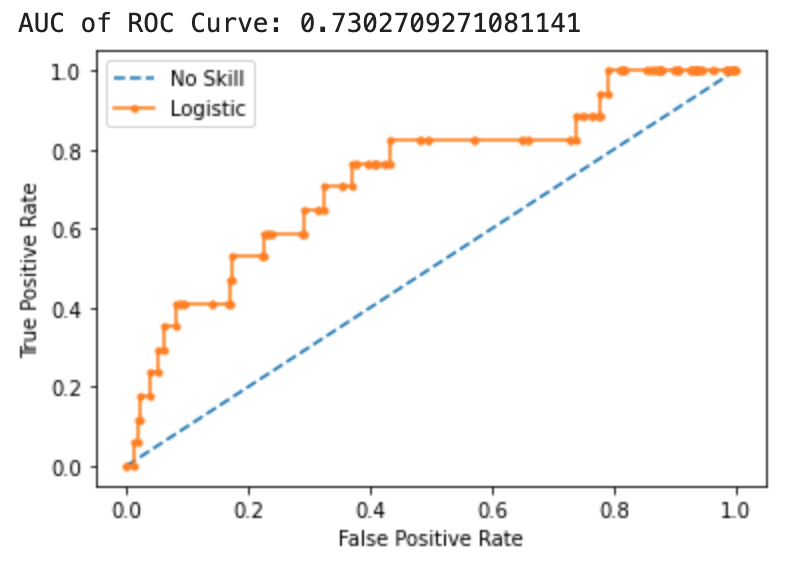
\includegraphics[scale=0.7]{roc1.png}
        	\end{center}
        	\legend{Fonte: trabalho nosso}
        \end{figure}
        
        \begin{figure}[htb]
        	\caption{\label{roc2}Curva ROC do modelo de predição de indicação, com seleção manual de atributos}
        	\begin{center}
        		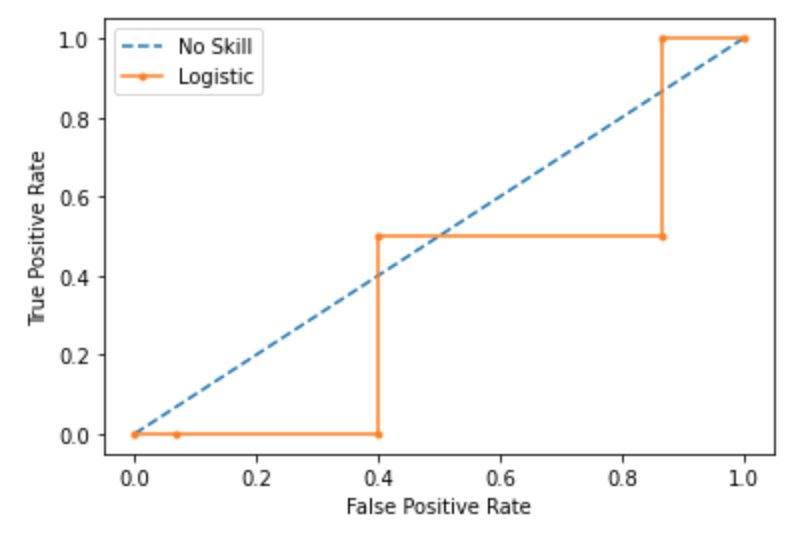
\includegraphics[scale=0.7]{roc2.png}
        	\end{center}
        	\legend{Fonte: trabalho nosso}
        \end{figure}
        
        % \begin{figure}[htb]
        % 	\caption{\label{roc3} Curva ROC do modelo de predição de vitória na categoria Best Picture, com seleção stepwise}
        % 	\begin{center}
        % 		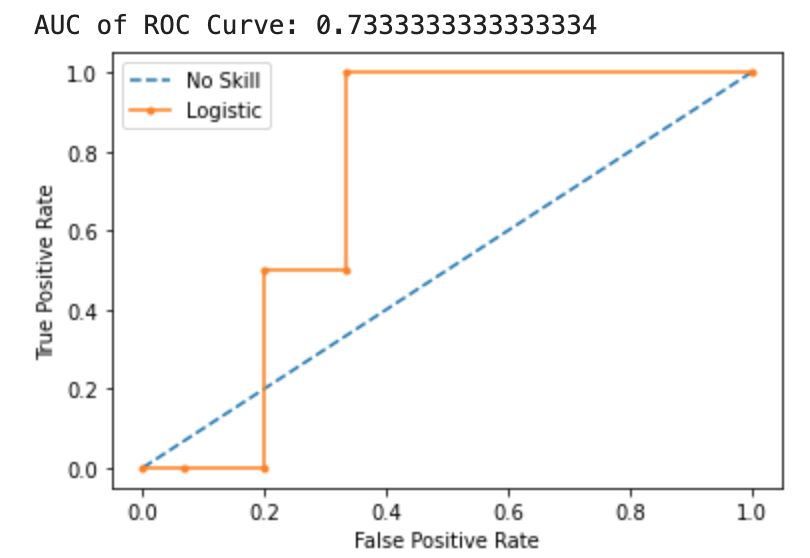
\includegraphics[scale=0.7]{roc3.png}
        % 	\end{center}
        % 	\legend{Fonte: trabalho nosso}
        % \end{figure}
        
        % \begin{figure}[htb]
        % 	\caption{\label{roc4}Curva ROC do modelo de predição de vitória na categoria Best Picture, com seleção manual de atributos}
        % 	\begin{center}
        % 		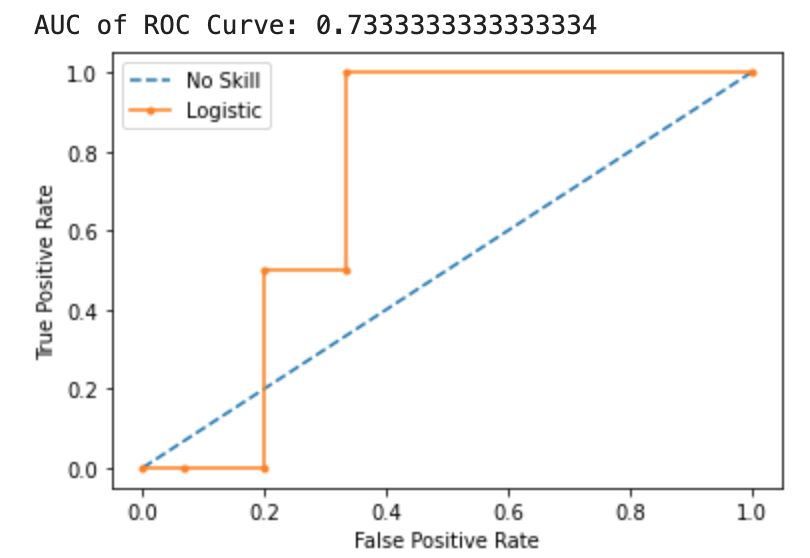
\includegraphics[scale=0.7]{roc4.png}
        % 	\end{center}
        % 	\legend{Fonte: trabalho nosso}
        % \end{figure}
        
        \begin{figure}[htb]
        	\caption{\label{confusao_1}Matriz de confusão do melhor modelo de predição de indicações}
        	\begin{center}
        		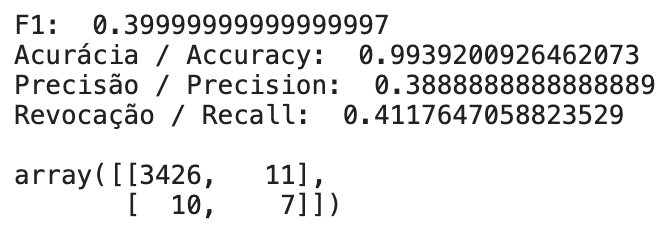
\includegraphics[scale=0.7]{confusao_1.png}
        	\end{center}
        	\legend{Fonte: trabalho nosso}
        \end{figure}
        
        \begin{figure}[htb]
        	\caption{\label{coefs_1}Coeficientes do melhor modelo de predição de indicações}
        	\begin{center}
        		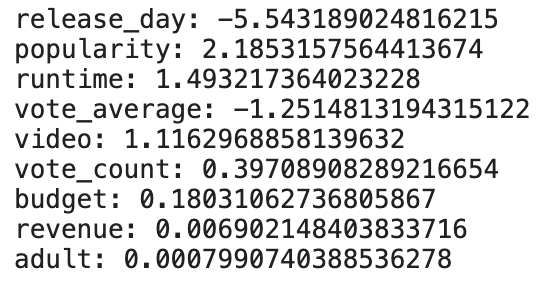
\includegraphics[scale=0.7]{coefs_1.png}
        	\end{center}
        	\legend{Fonte: trabalho nosso}
        \end{figure}
        
        Todos os modelos foram analisados por seus gráficos de curva ROC (figuras \ref{roc1} e \ref{roc2}). Como mostra a curva, o gráfico  do modelo 1 tem desempenho muito melhor que um classificador aleatório (ver \citeonline{mastery2021}). O mesmo não vale para o modelo 2, que em vários momentos tem desempenho pior que o modelo aleatório, e apenas para alguns thresholds apresenta desempenho pouquíssimo melhor.

        \subsection{Avaliação comparativa dos resultados}\par
        Para seleção do melhor threshold, foi utilizada a métrica de score f1. Incrementos de 0.01 foram feitos para thresholds entre 0 e 1, e o f1 score foi calculado para cada um dos thresholds. O threshold em que se obteve o melhor score f1 é considerado, em cada modelo, como o melhor threshold.
        
    \section{Resultados obtidos}
        
        O threshold com os melhores resultados para o modelo 1 foi de 0.15, com um f1 de 0.45. Com esse modelo, foi possível prever no conjunto de teste 7 verdadeiros positivos, com 11 falsos positivos e 9 falsos negativos, resultado bastante razoável num universo de 3454 instâncias de treinamento (figura \ref{confusao_1}).
        
        Já para o modelo 2, o melhor threshold encontrado foi de 0.33, com um f1 de 0.33. Com esse modelo, não foi possível prever no grupo de validação nenhum verdadeiro positivo, com 4 falsos positivos e 3 falsos negativos.(figura \ref{confusao_2})

        \subsection{Avaliação de importância dos metadados}\par
        A análise dos maiores coeficientes do modelo 1, em valor absoluto, revela a importância para o modelo de alguns critérios esperados, como data de lançamento, orçamento e renda. Alguns fatores menos óbvios que tiveram impacto no treinamento foram duração, se o filme foi lançado em vídeo, e se o filme é adulto ou não.(figura \ref{coefs_1})\par
        
        Para o modelo 2, em valor absoluto, os fatores que mais influenciaram o modelo foram, nessa ordem: se o filme foi lançado em vídeo, duração, média dos votos no Movie Lens, renda, popularidade no Movie Lens, adulto ou não-adulto e. orçamento.(figura \ref{coefs_2})\par

% Capítulo 4 - Conclusao
% ---
% Conclusão
% ---
\chapter[Conclusão]{Conclusão}
% ---
    \section{Interpretação dos resultados}\par
        Os resultados talvez fossem melhores não fosse pelo pequeno número de instâncias a serem analisadas ou mesmo à difícil predição do caráter humano da premiação, que é afetada pelos temas de cada filme, tendências artísticas e de conteúdo de cada ano, além de outras nuances sutis. Há que se considerar ainda a hipótese de que um outro modelo, com parâmetros mais bem ajustados, ou outro critério de seleção de atributos, obtivesse melhor resultado.
        
        Ainda que não sejam excelentes, os resultados apontam na direção de uma possibilidade de predição de filmes indicados ao Oscar. O modelo de regressão obteve um bom equilíbrio entre precisão e revocação, conseguindo prever um número considerável de verdadeiros positivos, sem incorrer em um grade número de falsos negativos ou falsos positivos.
        
        O modelo de predição de indicações ao Oscar condiz com a expectativa de que fatores conhecidos como data de lançamento, orçamento e renda tivessem grande influência, demonstrando ainda a importância de atributos menos esperados como duração, e se o filme é adulto ou não.
        
        De forma geral, os resultados apontam para a possibilidade de predição das chances de indicação de um filme, desde que conhecidas as variáveis acima. A questão das chances de vitória entre os indicados, por sua vez, permanece em aberto, já que os resultados ruins obtidos não são suficientes para concluir a impossibilidade dessa predição.

    \section[Dificuldades encontradas]{Dificuldades encontradas}

        Alguns dos problemas encontrados disseram respeito ao trabalho com dois datasets separados, um contendo dados da premiação do Oscar e outro com metadados dos filmes. Boa parte do esforço inicial do projeto se concentrou em formas de unir esses dois datasets. Mesmo assim, alguns dos filmes do dataset do Oscar não foram encontrados no dataset de metadados, e por isso foram deixados de fora. É razoável supor que o inverso aconteceu, e filmes no dataset de metadados não tiveram seus dados de premiação adicionados durante a integração de esquemas.
        
        A imprecisão de anos e nomes dos filmes, que utilizava formatos diferentes em cada dataset, e até mesmo inconsistentes dentro de um mesmo dataset, geraram grande dificuldade de associação entre os dados de um dataset e de outro. Por isso, a melhor hipótese talvez seja a criação e aprimoração de um dataset próprio para essa análise.
        
        No campo da metodologia, um problema recorrente ao longo da pesquisa foi o de definição do problema. Eventualmente, notamos que se tratava de pelo menos dois problemas - chances de indicação e de premiação -, com a grande diferença de que os dados de indicação são classe alvo no primeiro problema e atributos no segundo problema.
        
        Como as categorias não são mutuamente excludentes, pretendíamos ainda dividir cada um desses 2 problemas em 23, que é o número de categorias do Oscar, tentando analisar as chances de um filme em cada uma dessas categorias. O tamanho desse problema revelou-se excessivamente desafiador para essa pesquisa, que preferiu manter-se nas chances de indicação e premiação em uma única categoria (Oscar de melhor filme).
    
    \section[Próximas etapas da pesquisa]{Próximas etapas}
        Um subproduto possível da pesquisa é a criação do dataset unificado de metadados e indicações ao Oscar. A validação e consolidação desse dataset, ou a utilização de um dataset de metadados que já traga informações da premiação do Oscar, poderia gerar resultados melhores, e concentraria o esforço da pesquisa na possibilidade ou não de prever indicações, e com quais modelos.
        
        Próximos passos possíveis para a pesquisa também incluem a análise da predição com outros algoritmos além da regressão logística, e com expansão do problema para as outras categorias além de melhor filme.
        
        Os resultados mostram também um desempenho bastante consistente entre o modelo treinado com seleção stepwise de atributos e o treinado a partir da seleção manual de atributos que, intuitivamente, parecem relacionados às indicações. Uma investigação de subconjuntos possíveis dos atributos, e seus resultados, poderia revelar a existência de um ou mais atributos em comum que sejam determinantes na obtenção desses resultados.


% ---


% ----------------------------------------------------------
% ELEMENTOS PÓS-TEXTUAIS
% ----------------------------------------------------------
\postextual
% ----------------------------------------------------------

% -----------------------------------------------------------
% Referências bibliográficas
% ----------------------------------------------------------
\bibliography{fim0-bibliografia}


% ----------------------------------------------------------
% Glossário
% ----------------------------------------------------------
%
% Consulte o manual da classe abntex2 para orientações sobre o glossário.
%
%\glossary

% ----------------------------------------------------------
% Apêndices
% ----------------------------------------------------------
%%% USPSC-Apendice.tex
% ---
% Inicia os apêndices
% ---

\begin{apendicesenv}
% Imprime uma página indicando o início dos apêndices
\partapendices
\chapter{Apendice(s)}


\end{apendicesenv}
% ---

% ----------------------------------------------------------
% Anexos
% ----------------------------------------------------------
%%% USPSC-Anexos.tex
% ---
% Inicia os anexos
% ---
\begin{anexosenv}

% Imprime uma página indicando o início dos anexos
\partanexos

% ---
\chapter{Anexo}
% ---


\end{anexosenv}


%---------------------------------------------------------------------
% INDICE REMISSIVO
%--------------------------------------------------------------------
%%% USPSC-IndicexRemissivos.tex
% ---
% Inicia os Índices Remissivos
% ---
%---------------------------------------------------------------------
% INDICE REMISSIVO
%--------------------------------------------------------------------
\phantompart
\printindex
%---------------------------------------------------------------------


%---------------------------------------------------------------------

\end{document}
